\documentclass{article}
\usepackage[utf8]{inputenc}
\usepackage{geometry}
\geometry{left=2.0cm,right=2.0cm,top=2.5cm,bottom=2.5cm}
\usepackage{amsmath, amsthm, amssymb, bm, bbm}
\usepackage{mathrsfs}
\usepackage{extarrows}
\usepackage{pifont}
\usepackage{diagbox}
\usepackage{xcolor}
\usepackage{multirow}
\usepackage{graphicx}
\usepackage{hyperref}
\usepackage{float}
\hypersetup{colorlinks=true, linkcolor=blue, citecolor=blue, urlcolor=black}
\usepackage{caption}
\usepackage{braket}
\usepackage{pgfplots}
\usepackage{multirow}
\usepackage{authblk} 
\usepackage{tikz}
\usepackage{cite}
\usepackage{qcircuit}
\usepackage{physics}
\usepackage{array}
\usepackage{bbm}

\newtheorem{theorem}{Theorem}
\newtheorem{lemma}{Lemma}
\newtheorem{proposition}{Proposition}
\newtheorem{problem}{Problem}
\newtheorem{corollary}{Corollary}
\newtheorem{claim}{Claim}
\newtheorem{conjecture}{Conjecture}
\newtheorem{definition}{Definition}
\newtheorem{fact}{Fact}
\newtheorem{construction}{Construction}
\newtheorem*{answer}{Answer}
\newtheorem*{example}{Example}
\newtheorem*{counterexample}{Counterexample}
\newtheorem{assumption}{Assumption}


\allowdisplaybreaks[2]



\newcommand{\ii}{\mathsf{i}}
\newcommand{\Twhole}{T^{(\text{whole})}}
\newcommand{\Tcouple}{T^{(e)}_{\mathcal{P}_\frac{n}{2}} T^{(o)}_{\mathcal{P}_\frac{n}{2}}}
\newcommand{\polylog}{\mathrm{polylog}}
\newcommand{\alpl}{\alpha_{\{\gamma_i\gamma_j\}, 2t+1}^{\mathscr{L}}}
\newcommand{\alpr}{\alpha_{\{\gamma_i\gamma_j\}, 2t+1}^{\mathscr{R}}}
% \newcommand{\span}{\mathrm{span}}
% \newcommand{\dd}{\mathsf{d}}

% \newcommand{\abs}[1]{\left| #1 \right|}
% \newcommand{\var}[1]{\mathrm{Var}\left[#1 \right]}
\newcommand{\supket}[1]{|#1 \rangle\rangle}
\newcommand{\supbra}[1]{\langle\langle #1 |}
\newcommand{\supketbra}[2]{
    \supket{#1 } \supket{#1 } \supbra{#2} \supbra{#2} 
}
\newcommand{\floor}[1]{\lfloor #1 \rfloor}
\newcommand{\mean}{\mathop{\mathbb{E}}}
\newcommand{\Var}{\mathop{\mathrm{Var}}}

\begin{document}
% \title{Optimized-depth fermionic classical shadow}
% \author{Kaiming Bian}
% \affiliation{Shenzhen Institute for Quantum Science and Engineering,
% Southern University of Science and Technology, Shenzhen 518055, China}
% \affiliation{International Quantum Academy, Shenzhen 518048, China}
% \affiliation{Guangdong Provincial Key Laboratory of Quantum Science and Engineering, Southern University of Science and Technology, Shenzhen, 518055, China}
% \author{Bujiao Wu}
% \affiliation{Shenzhen Institute for Quantum Science and Engineering,
% Southern University of Science and Technology, Shenzhen 518055, China}
% \affiliation{International Quantum Academy, Shenzhen 518048, China}
% \affiliation{Guangdong Provincial Key Laboratory of Quantum Science and Engineering, Southern University of Science and Technology, Shenzhen, 518055, China}
\section{Introduction}
% \section{Theory}

\section{Preliminary: Fermionic Classical Shadow}

\subsection{Majorana operators and matchgate circuits}

Studying Majorana operators in Fermionic systems is essential due to their role as quasiparticles that are their own antiparticles, which makes the Majorana operators as fundamental research objects in Fermionic systems. The Majorana operators are usually defined as 
\begin{equation}
    \gamma_{2 j-1}:=a_j+a_j^{\dagger}, \quad \gamma_{2 j}:=-\ii\left(a_j-a_j^{\dagger}\right)
    \label{eq: standard Majorana operators}
\end{equation}
corresponding to the ladder operators $a_j$. In a system with $n$ different modes, we will obtain $2n$ Majorana operators. The fundamental properties of Majorana operators are that they are Hermitian and satisfy the anti-commutation relations
\begin{equation}
    \{\gamma_\mu, \gamma_\nu\} = 2 \delta_{\mu, \nu} \mathbbm{1},
    \label{eq: anti-commutation relation of majorana operators}
\end{equation}
where $\mu, \nu \in [2n]$, $[2n]:= \{1,2,3,\cdots, 2n\}$. Observables in fermionic systems can be expressed as products of Majorana operators~\cite{hackl2021bosonic}. Therefore, it is natural to study the product of Majorana operators 
\begin{equation}
    \gamma_S := \gamma_{\mu_1}\gamma_{\mu_2}\cdots\gamma_{\mu_{|S|}},
\end{equation}
where $\mu_1 < {\mu_2}< \cdots < \mu_{|S|}$, and $S = \{\mu_1 , {\mu_2}, \cdots , \mu_{|S|}\}$. Especially, we set $\gamma_\emptyset$ to the identity operator $\mathbbm{1}$ if $S$ is the empty set $\emptyset$.


% We could get different set of 
In general, we consider a set of operators that satisfy the anti-commutation relation \eqref{eq: anti-commutation relation of majorana operators} as a set of Majorana operators. A different set of Majorana operators can be obtained by the orthogonal transformation of the standard Majorana operators
\begin{equation}
    \tilde{\gamma}_\mu=\sum_{\nu=1}^{2 n} Q_{\mu \nu} \gamma_\nu,
\end{equation}
where $Q$ is a real orthogonal matrix, $Q \in O(2n)$, and $\gamma_\nu$ is the standard Majorana operators defined in \eqref{eq: standard Majorana operators}.
The $\tilde{\gamma}_\mu$ satisfy the anti-commutation relation \eqref{eq: anti-commutation relation of majorana operators}, which means the set of $\tilde{\gamma}_\mu$ is a valid choice of Majorana operators. 

% Now, let us consider the operators which preserve the condition of Majorana operators. 
The fermionic Gaussian unitaries are the unitaries which preserve the anti-commutation relation~\cite{hackl2021bosonic, weedbrook2012gaussian,wang2007quantum}. 
In other words, the fermionic Gaussian unitaries $U_Q$ transform one Majorana operator $\gamma_\mu$ to an another Majorana operator $\tilde{\gamma}_\mu$
\begin{equation}
 U_Q^{\dagger} \gamma_\mu U_Q=\sum_{\nu=1}^{2 n} Q_{\mu \nu} \gamma_\nu = \tilde{\gamma}_\mu.
\end{equation}
Similarly, the fermionic Gaussian unitaries preserve the product of Majorana operators $\gamma_S$ as well
\begin{equation}
 U_Q^{\dagger} \gamma_S U_Q=\sum_{|S'| = S} \xi_{S'} \gamma_{S'},
\end{equation}
where $\xi_{S'}$ are real coefficients, and $S' \subset [2n]$.

The matchgate circuits are the counterpart of fermionic Gaussian unitaries in qubits representation. In qubits representation, we express the fermionic Gaussian unitaries in terms of Pauli operators and quantum circuits via the Jordan-Wigner transformation
\begin{equation}
    \gamma_{2 j-1}=\left(\prod_{i=1}^{j-1} Z_i\right) X_j, \quad \gamma_{2 j}=\left(\prod_{i=1}^{j-1} Z_i\right) Y_j.
\end{equation}
The Jordan-Wigner transformation builds the bridge between Majorana operators and Pauli operators, which enables us to express $U_Q$ by Pauli operators. Firstly, the two-qubit matchgates could be expressed by two-qubit $X$-rotations and single-qubit $Z$ rotations
\begin{equation}
    M_2 = \left\{\prod_j\exp(\ii \theta_1^j  Z\otimes \mathbbm{1} + \ii \theta_2^j  \mathbbm{1}\otimes Z)\exp(\ii \theta_3^j  X\otimes X)\mid \theta^j_k \in \mathbb{R}, k = 1,2,3 \right\}.
\end{equation}
The $n$-qubits matchgate circuit could be implemented by interweavely applying two-qubits matchgates. The group of $n$-qubits matchgate circuits is denoted as $M_n$, which is called the matchgate group. Here is an example of implementing $U_Q\in M_4$ via interwoven two-qubits matchgates, which is shown in Fig.~\ref{fig:1}.

\begin{figure}
    \centering
    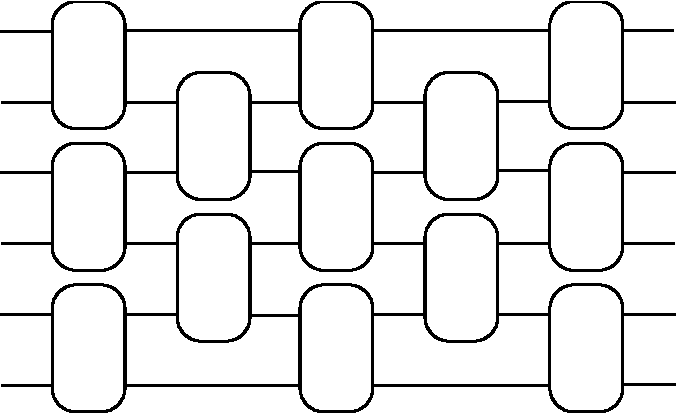
\includegraphics[width=0.5\linewidth]{figures/main/matchgate.pdf}
    \caption{The quantum circuit for constructing $U_{Q_d}$. Each two-qubit gate is randomly drawn from Gaussian group $M_2$ independently. A standard circuit we set contains an even number of qubits and an odd number of layers.}
    \label{fig:1}
\end{figure}

% \begin{equation}
% \Qcircuit @C=1em @R=0.3em {
%     & \multigate{1}{U_Q^{(1)}} & \qw & \multigate{1}{U_Q^{(4)}} & \qw\\
%     & \ghost{U_Q^{(1)}} & \multigate{1}{U_Q^{(3)}}& \ghost{U_Q^{(4)}} & \qw \\
%     & \multigate{1}{U_Q^{(2)}} & \ghost{U_Q^{(3)}}& \multigate{1}{U_Q^{(5)}} &\qw \\
%     & \ghost{U_Q^{(2)}} & \qw &\ghost{U_Q^{(5)}} &\qw\\
% }
% \end{equation}
where $U_Q^{(i)}$ is two-qubits matchgate. In this work, we will always consider the implementation of $U_Q$ as a circuit of interwoven two-qubits matchgates. 


 
\subsection{Fermionic classical shadow protocal}
% 回顾一下Classical shadow
Classical shadows is a method in quantum information that allows for efficient estimation of properties of quantum states with fewer measurements than quantum state tomography~\cite{huang2020predicting}. The process involves randomly applying a Clifford gate $U$ to a quantum state $\ket{\psi}$. After applying these transformations, measurements are taken, yielding outcomes $\ket{b}$ that form a classical description or ``shadow" $\mathcal{M}^{-1}(U^\dagger \ketbra{b}{b} U)$ of the original quantum state $\ket{\psi}$. Each classical shadow contains a piece of the information of the original state, and the average of shadows could rebuild the original state~\cite{huang2020predicting}
\begin{equation}
\ketbra{\psi}{\psi}
=\mathbb{E}\left[\mathcal{M}^{-1}\left(U^{\dagger} \ketbra{b}{b} U\right)\right].
\label{eq: mean value of classical shadow}
\end{equation}
Averaging the shadows can be efficiently processed on a classical computer because of Gottesman–Knill theorem. In contrast to the exponential sample complexity required in quantum state tomography, the classical shadows protocol requires only polynomial measurements to reconstruct the state, demonstrating a significant advantage. 


The concept of classical shadows has been extended to fermionic systems~\cite{wan2022matchgate}, referred to as fermionic classical shadows (FCS). In fermionic systems, the physical operators must satisfy fermionic parity~\cite{bravyi2002fermionic, o2018majorana}. Not all Clifford gates are valid operators in these systems, prompting researchers to use matchgate circuits instead. This is because matchgate circuits preserve fermionic parity~\cite{jozsa2008matchgates, hebenstreit2020computational, cai2009theory}.
Fermionic classical shadows follow the protocol of original classical shadows but replace the random Clifford gate with random matchgates circuits.


% 描述FCS 与CS的异同:1、子空间可逆  2、 mean value
% Similar to classical shadows, the original state could be rebuilt from the classical shadow in FCS, which means the FCS is an unbias estimation.
Similar to traditional classical shadows, the original state $\ket{\psi}$ could be reconstructed from the classical shadows $\mathcal{M}^{-1}\left(U^{\dagger} \ketbra{b}{b} U\right)$ in FCS, and the reconstruction is efficient for classical computer~\cite{wan2022matchgate}. This fact means that the FCS provides an unbiased estimation of the original state.
However, the channel $\mathcal{M}$ is not invertible in the whole Hilbert space. It is only invertible in the subspace which is spanned by even operators
\begin{equation}
    \Gamma_{\text{even}} := \mathrm{span}\{ \gamma_S \mid |S| = 2j, j=0,1,2,\cdots \}.
\end{equation}
In other words, $\mathcal{M}(\gamma_S) = 0$ for odd cardinal number $|S| = 2j+1$. Unless otherwise specified, we will focus on the space of $\Gamma_{\text{even}}$. 

Compared to traditional quantum state measurement methods, the advantage of the classical shadows approach depends on the number of required measurements, known as the sample complexity. The sample complexity is a crucial indicator for estimating the performance of a protocol. We consider an estimation protocol efficient if it requires only a polynomial number of measurements to approximate the expectation value of an observable. 
Traditional quantum state tomography requires an exponential number of measurements to reconstruct the state, making it inefficient. For FCS, efficiency depends on the observable. Ref.~\cite{wan2022matchgate} demonstrates that estimation is efficient if the observable is $\gamma_S$ with a constant cardinality $|S|$. In contrast, it is inefficient if $|S|$ is of the order $\mathcal{O}(n)$.
% Ref.~\cite{wan2022matchgate} gives the variance of the FCS estimator. 

\section{Relatively shallow fermionic classical shadows}

% variance 的表达式、跟深度的关系、无穷阶的理论结果


% % Compared to traditional quantum state measurement methods, the advantage of the classical shadows approach depends on the required number of measurements. 
% % This number is generally referred to as the sample complexity. 
% % Thus, the sample complexity of FCS becomes a crucial indicator of its performance. 

% We consider an estimating protocol to be efficient if it only needs a polynomial number of measurements to approximate the expectation value of an observable. 
% The traditional quantum state tomography needs an exponential number of measurements to rebuild the state, which means it is inefficient. When it comes to FCS, whether FCS is efficient depends on the observable. Ref.~\cite{wan2022matchgate} shows that the estimation is efficient if the observable is $\gamma_S$ with constant cardinal number $|S|$. In contrast, the estimation is inefficient if the cardinal number $|S|$ has the order $\mathcal{O}(n)$.




% If polynomial number of measurements is needed to approximate the expected value of an observable, we consider this measurement to be efficient.
% 如果只需要多项式次测量就能逼近观测量的期望值,我们就称这个测量是有效的。

% Due to the sampling distribution and Chebyshev inequality, the sample complexity is determined by the variance of the estimator. 

The FCS requires a random sampling in the $t$-design of the matchgate circuit. Generally, any matchgate circuit can be created within $\mathcal{O}(n^2)$ depth~\cite{jiang2018quantum}, which implies that a Haar random circuit ensemble requires $\mathcal{O}(n^2)$ depth circuit to construct. 
However, for certain specific observables, we do not need deep circuits to construct a $t$-design of matchgate circuits. In this case, the constructed shallow circuit ensemble may not form a unitary design, but it is deep enough to estimate the expected value. One extreme example is predicting the expectation value of observables $ \gamma_i\gamma_{i+1} = Z_i$. The expectation could be an efficient estimation by direct measurement on the computational basis without extra construction of a random $t$-design matchgate circuit. This fact motivates us to study the relatively shallow fermionic classical shadows (RSFCS).


In this section, we explore the properties of RSFCS, especially estimating the order of circuit depth required to ensure that the final sample complexity remains polynomial. We give the relationship between the one-reduced density matrix ($1$-RDM) and the required depth of circuit under the reasonable assumption. 


% Here, we take an extreme example to illustrate the point. 
% The expectation value $\langle \gamma_1\gamma_2 \rangle = \langle Z_1 \rangle$ could be an efficient estimation by direct measurement on the computational basis without extra construction of a random $t$-design matchgate circuit.
% If the observable is $\gamma_1\gamma_2 = Z_1$, the expectation
% 然而,对于一些特殊的观测量而言,我们并不需要很深的线路去构造 $t$-design of matchgates circuit




% In this section, we aim to estimate the order of circuit depth required to ensure that the final sample complexity remains polynomial. We give the relationship between the one-reduced density matrix ($1$-RDM) and the required de
% 在合理的假设下, 且$|S|=2$ 时, 观测量gammaS与保持有效性所需的深度之间的关系

% 这里,我们想要估计如果想要保持最后的sample complexity 是多项式深的条件下,所需要的线路深度是多少这个问题
\subsection{Shadow channel in RSFCS}
\label{sec: shadow channel}
% In RSFCS, we apply $d$ layers of interwoven two-qubit matchgates, then measure the circuit in computational basis
In RSFCS, 
The unitary ensemble consists of $ d$ layers of interwoven two-qubit matchgates. Each two-qubit matchgates is Haar randomly drawn from the matchgate group $M_2$.
The shadow channel $\mathcal{M}_d(\rho)$ is given by
\begin{equation}
    \mathcal{M}_d(\rho) := \sum_b \dd U_{Q_d} \bra{b}U_{Q_d} 
  \rho U_{Q_d}^\dagger \ket{b} \rho U_{Q_d}^\dagger \ket{b} \bra{b}U_{Q_d},
\end{equation}
where the $U_{Q_d}$ is a unitary in a $d$-layers ensemble. We show that the shadow channel could be diagonalized by Majorana operators:
\begin{lemma}
\label{lemma 1}
The shadow channel in RSFCS has the property
\begin{equation}
\mathcal{M}_d(\gamma_S) = \alpha_{S,d} \gamma_S,
\end{equation}
where 
$\alpha_{S,d} = \int \dd U_{Q_d} \abs{\bra{0}U_{Q_d} \gamma_S U_{Q_d}^\dagger\ket{0}}^2.$
\end{lemma}

Lemma \ref{lemma 1} tells that the RSFCS is an unbias estimation because 
\begin{equation}
    \mathop{\mathbb{E}}\limits_{U_{Q_d}, b } ( \mathcal{M}^{-1}_{d}(U_{Q_d}^\dagger \ket{b} \bra{b}U_{Q_d})) = \mathcal{M}^{-1}_{d}(\mean(U_{Q_d}^\dagger \ket{b} \bra{b}U_{Q_d}) ) = \rho.
\end{equation}



% \subsection{The variance of FCS estimation}
Due to the sampling distribution and Chebyshev inequality, the sample complexity is determined by the variance of the estimator. The variance of the RSFCS could be bounded by $\frac{1}{\alpha_{S,d}}$:
\begin{lemma}
\label{lemma 2}
Given any observable $\gamma_S$ and an unknown quantum state $\rho$, let $v$ be the estimation of $\tr(\rho \gamma_S)$ with shadow channel $\mathcal{M}_d$.
Then the variance in the average of the input state can be bounded to $1/\alpha_{S,d}$,
\begin{equation}
    \Var[v]\leq \frac{1}{\alpha_{S,d}}.
\end{equation}
\end{lemma}

Notice that the bond is tight because there always exist certain states $\rho$ such that the expectation value of $v$ is $0$, $\mean[v] =0$. In this case, the variance of $v$ is described by $\frac{1}{\alpha_{S,d}}$. Then, the order of $\alpha$ will directly determine the order of the variance. 
And we will estimate the order of $\alpha_{S,d}$ in certain cases. 






% \subsection{Computing measurement channel is efficient}
% In this section, we will demonstrate that the post-processing of RSFCS is effective. The property ensures that the whole process of RSFCS is an effective method. Concretely, the expectation value of classical shadows $\tr (\mathcal{M}_d^{-1}(U_{Q_d}^\dagger \ket{b} \bra{b}U_{Q_d})\gamma_S)$ should be effectively reconstructed after obtaining the measurement $\ket{b}$. 

% The calculation of $U_{Q_d}^\dagger \ket{b} \bra{b}U_{Q_d}$ is effective. The set $M_n \cap \mathrm{Cl}_n$ is a $3$-design of the Gaussian unitary group, where $\mathrm{Cl}_n$ is the $n$-qubit Clifford group. Thus, the calculation of $U_{Q_d}^\dagger \ket{b} \bra{b}U_{Q_d}$ could be considered as sampling dozens of unitary from the ensemble $M_2 \cap \mathrm{Cl}_2$ and then interweavely apply the unitary to a stabilizer state. Due to the Gottesman–Knill theorem, classical computer can efficiently apply one such unitary on a stabilizer state. 
% It only needs polynomial number of layers to create a $3$-design of $M_n$, which means that the number of all two-qubit unitaries is polynomial. 
% Applying polynomial numbers of such unitaries to the measured state $\ket{b}$ is efficient. 

% According to Lemma \ref{lemma 1}, the $\mathcal{M}_d$ could be diagonalized by Majorana operators, which means $\mathcal{M}_d$ is a Hermitian operator, 
% \begin{equation}
%     \tr (\mathcal{M}_d^{-1}(U_{Q_d}^\dagger \ket{b} \bra{b}U_{Q_d})\gamma_S) = \tr (U_{Q_d}^\dagger \ket{b} \bra{b}U_{Q_d}\mathcal{M}_d^{-1}(\gamma_S)) = 
%     \frac{1}{\alpha_{S,d}} \tr (U_{Q_d}^\dagger \ket{b} \bra{b}U_{Q_d}\gamma_S).
% \end{equation}
% Each Majorana operator $\gamma_S$ is correspond to a Pauli operator by Jordan-Wigner transformation. The trace of a stabilizer state $U_{Q_d}^\dagger \ket{b} \bra{b}U_{Q_d} $ and another Pauli operator is efficient. Thus, the classical post-processing is efficient if the coefficient $\alpha_{S,d}$ could be computed efficiently.

% \begin{lemma}
% \label{lemma 3}
%     The calculation of $\alpha_{S,d}$ could be represented by a tensor network.
% \end{lemma}

% \begin{proof}(Sketch of the proof)
%     Lemma \ref{lemma 1} gives the definition of the $\alpha_{S,d}$, which is an integral of unitary $U_{Q_d}$. The integral over $U_{Q_d}$ can be broken down into an integral over each two-qubit matchgates, which has the closed form. 
    
% The detail of the proof is shown in the Appendix.
% \end{proof}

% The 

\subsection{Represent $\alpha_{S,d}$ in tensor network}
In Sec.~\ref{sec: shadow channel}, we demonstrated that the number of samples needed is represented by the variable $\alpha_{S,d}$. Put another way, how quickly the required sample size increases depends on how quickly $\alpha_{S,d}$ gets smaller. If $\alpha_{S,d}$ is in the order of $\frac{1}{\mathrm{poly}(n)}$, the sample complexity scales proportionally to a polynomial of qubit number $n$. Otherwise, if $\alpha_{S,d}$ becomes exponentially small, then the protocol requires exponential samples and is ineffective for practical use as $n$ becomes larger.

The RSFCS devolves to FCS when the layer number $d$ goes to infinite. In this case, the $U_{Q_\infty}$ is Haar randomly drawn from Gaussian group $M_n$. Even FCS is not always efficient. 
FCS is inefficient for $k$-RDM with large $k$. The reduced density matrix of $k$ particle in a fermionic system could be expressed by a linear combination of $\gamma_S$ with $|S| = 2k$. For instance, the $\alpha_{S,\infty}$ is exponentially small if $k$ is appropriated to the scale of the whole system $n$~\cite{zhao2021fermionicpartial}. 
Thus, we need to estimate the order of $\alpha_{S,d}$ to check if the RSFCS is efficient. Here, we use tensor network to calculate the $\alpha_{S,d}$:
\begin{lemma}
\label{lemma 3}
    The calculation of $\alpha_{S,d}$ could be represented by a tensor network.
\end{lemma}

Here, we show the sketch of the proof, and the details of the proof are shown in the Appendix.~\ref{appendix 3}. We will represent the Majorana operators $\gamma_S$ and the unitary transformation of the Majorana operators $U_{Q_d} \gamma_S U_{Q_d}^\dagger$ as the super vectors $\supket{\gamma_S}$ and the super operators $\mathcal{U}_{Q_d}$,
\begin{equation}
   \left(U_{Q_d} \gamma_S U_{Q_d}^\dagger \right) \otimes \left(U_{Q_d} \gamma_S U_{Q_d}^\dagger \right) \to \mathcal{U}_{Q_d} \supket{\gamma_S, \gamma_S}.
\end{equation}
The $\alpha_{S,d}$ could be expressed in terms of the super vectors and the super operators
\begin{equation}
\label{eq: alpha to tensor}
    \alpha_{S,d} 
    = \supbra{0,0}  \int \dd U_{Q_d} \mathcal{U}_{Q_d} \supket{P^S,P^S},
\end{equation}
where $P^S$ is the Pauli operator that corresponds to the Majorana operator $\gamma_S$ by Jordan-Wigner transformation. The state $\supket{P^S,P^S}$ is the 
super operator of $P^S \otimes P^S$.
Notice that the integral over $U_{Q_d}$ can be broken down into an integral over each two-qubit matchgates
\begin{equation}
    \int \dd U_{Q_d} \mathcal{U}_{Q_d} = \int \dd U_{Q_2}^{(1)} \mathcal{U}_{Q_2}^{(1)} \int \dd U_{Q_2}^{(2)} \mathcal{U}_{Q_2}^{(2)} \cdots\int \dd U_{Q_2}^{(m)} \mathcal{U}_{Q_2}^{(m)},
\end{equation}
where $U_{Q_2}^{(j)}$ is the $j$-th two-qubit matchgate, and the $m$ is the total number of two-qubit matchgate. Each Integral of two-qubit matchgates $U_{Q_2}^{(i)}$ equals to another, because matchgates $U_{Q_2}^{(i)}$ are sampled from the Gaussian unitary group $M_2$ independently. Thus, we could denote all integrals of two-qubit matchgates as a 4-bond tensor
\begin{equation}
% \label{eq: definition of T}
    T^{\sigma_1, \sigma_2}_{~~\sigma_3, \sigma_4} = \supbra{\sigma_1, \sigma_2}\supbra{\sigma_1, \sigma_2}\int \dd U_{Q_2}^{(i)} \mathcal{U}_{Q_2}^{(i)} \supket{\sigma_3, \sigma_4}\supket{\sigma_3, \sigma_4},
\end{equation}
where $\sigma_1, \sigma_2, \sigma_3, \sigma_4$ are two-qubits Pauli operators. 
Therefore,  the $\alpha_{S,d}$ in Eq.~\eqref{eq: alpha to tensor} could be represented by a contraction of tensors $T$, which is shown in Fig.~\ref{fig:TNcoefRep}.

\begin{figure}
    \centering
    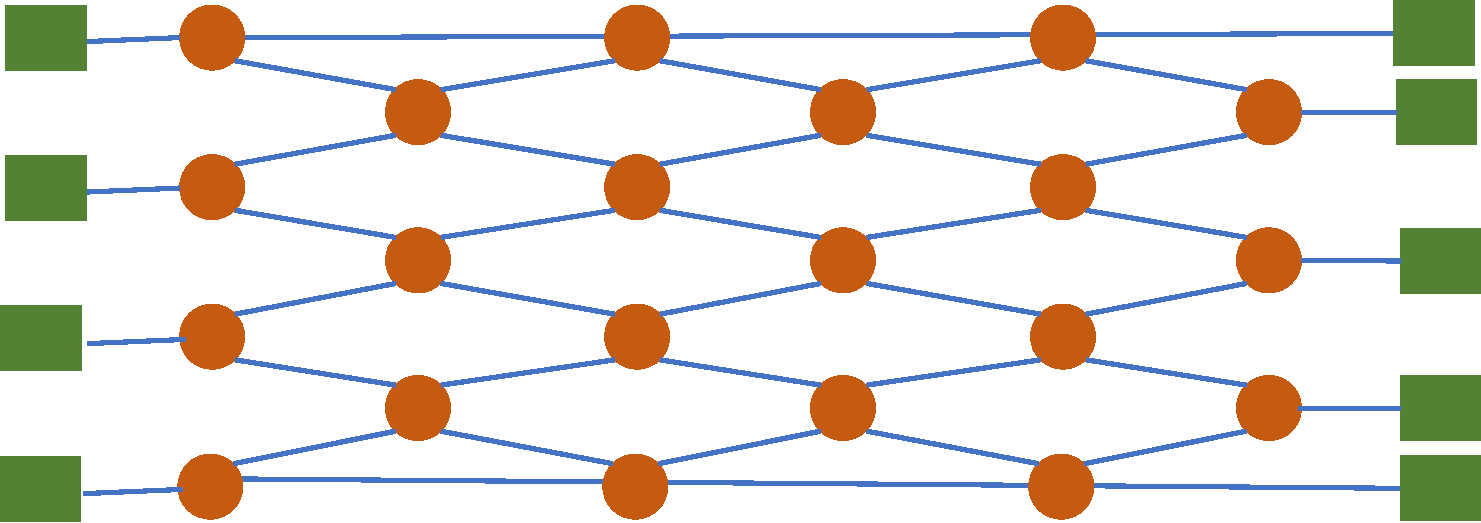
\includegraphics[width = 0.8\textwidth]{shallowCStensor_rep.pdf}
    \caption{Tensor network representation of the twirled $d$-layers matchgate circuit.}
    \label{fig:TNcoefRep}
\end{figure}
    
% The detail of the proof is shown in the Appendix.

\subsection{Required depth for 1-RDM}

We know the order of $\alpha_{S, d}$ in extreme cases. For the RSFCS with constant $k$, when the depth is $0$, the $\alpha_{S, 0}$ equals $0$ for certain observables; and when the depth goes to infinity, the RSFCS devolves to FCS and the $\alpha_{S, \infty}$ is in the order of $\frac{1}{\mathrm{poly}(n)}$. Therefore, there must be some threshold in between, which maintains polynomial sample complexity with relatively shallow depth. 

Estimating this order using tensor network contraction in mesoscopic depth is challenging. However, we could simplify the calculation by restricting the action of the tensor within the subspace spanned by $1$-RDM. The subspace spanned by $k$-RDM is an invariant subspace for Gaussian unitary $U_{Q_d}$ because the evolution of Gaussian operators transforms a $k$-RDM to another $k$-RDM with the same $k$. 

% We map the contraction of the tensor network to a random walk over a 2D lattice. 
By restricting the action of $U_{Q_d}$ to the subspace spanned by $1$-RDM, we can introduce more refined structures by mapping this subspace to a polynomial space. This isomorphism allows us to analyze the system more effectively. In this context, the tensor network contraction of $\alpha_{S,d}$ is equivalent to a random walk in the polynomial space. More importantly, after setting the circuits in a standard form (see Fig.~\ref{fig:1}), the effective subspace can be further reduced. This reduced space becomes simple enough to reveal some hidden phenomena.


% 限制在子空间后,我们可以找到这个子空间上的一组基。这组基是由Pauli基表述的
% 我们可以将U 的作用限制在子空间上之后,为了引入更精细的结构,我们将这个子空间同构于一个多项式空间。在原空间上U的作用等价于在新的空间上的随机游走。

\begin{lemma}
    Let the qubit number $n$ be an even number, and the number of layers $d$ be an odd number. The action of $U_{Q_d}$ on the standard circuit could be represented in the space of the quadratic polynomial with $\frac{n}{2}$ elements. 
\end{lemma}

Here we demonstrate the idea of the lemma and leave the details in the Appendix \ref{sec: Mapping the action of tensors to random walk}. We observe that the state $\mathcal{U}\supket{P^S}^{\otimes 2}$ could be expressed by the linear combination of the following super vectors
\begin{equation}
\begin{aligned}
    & \supket{Z_{2i-1}} + 4\sum_{M_{2i-1}, M_{2i}} \supket{M_{2i-1}M_{2i}} +  \supket{Z_{2i}}  & & \longmapsto y_i^2\\
    & 
    \begin{aligned}
        &\sum_{M_{2i-1}, M_{2j-1}}\supket{M_{2i-1}(\prod_{k = 2i}^{2j-2} Z_k) M_{2j-1}} + \sum_{M_{2i}, M_{2j-1}}\supket{M_{2i}(\prod_{k = 2i+1}^{2j-2} Z_k) M_{2j-1}} \\
        +&\sum_{M_{2i-1}, M_{2j}}\supket{M_{2i-1}(\prod_{k = 2i}^{2j-1} Z_k) M_{2j}} + \sum_{M_{2i}, M_{2j}}\supket{M_{2i}(\prod_{k = 2i+1}^{2j-1} Z_k) M_{2j}}
    \end{aligned}
      & & \longmapsto y_i y_j, i< j\leq \frac{n}{2} ,
\end{aligned}
\label{eq: basis transform}
\end{equation}
where the summation is with respect to indices $M$ over the Pauli operators $X$ and $Y$. For example,
\begin{equation*}
    \sum_{M_{2i-1}, M_{2i}\in \{X,Y\}} \supket{M_{2i-1}M_{2i}} = \supket{X_{2i-1}X_{2i}} + \supket{X_{2i-1}Y_{2i}} + \supket{Y_{2i-1}X_{2i}} + \supket{Y_{2i-1}Y_{2i}}.
\end{equation*}
The supervectors in Eq.~\eqref{eq: basis transform} forms the basis of the subspace $\mathrm{span}\{\mathcal{U}_{Q_d} \supket{\gamma_S, \gamma_S}\mid |S| = 2\}$. In order to introduce a more manageable structure for manipulation and to facilitate a clearer expression, we establish a correspondence between these states and the basis in an $\frac{n}{2}$ variable quadratic polynomial space $\mathcal{P}_\frac{n}{2}$. The rule of correspondence is described in Eq.~\eqref{eq: basis transform}. 

\begin{figure}
    \centering
    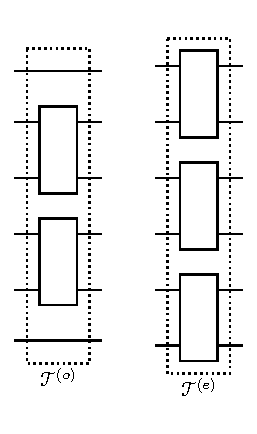
\includegraphics[width=0.22\linewidth]{figures/appendix/Todd_Teven.pdf}
    \caption{The odd layer $T^{(o)}$ and the even layer $T^{(e)}$. }
    \label{fig: odd layer and even layer}
\end{figure}



The tensor $\int \dd U_{Q_d} \mathcal{U}_{Q_d}$ could be expressed by alternately apply $T^{(o)}$ and $T^{(e)}$ gates, 
\begin{equation}
\Twhole := \int \dd U_{Q_d} \mathcal{U}_{Q_d}=\left(\prod_{i=0}^{t} T^{(e)} T^{(o)}\right) T^{(e)}, 
\end{equation}
where $d= 2t+1$ stands for the number of layers, $T^{(o)}$ is the odd layer which shown in Fig.~\ref{fig: odd layer and even layer}, similar as $T^{(e)}$.  Based on Eq.~\ref{eq: basis transform}, we can find the unique correspondence of $T^{ (e)} \supket{\gamma_S, \gamma_S}$ to $y_iy_j$ in the space $\mathcal{P}_\frac{n}{2}$.
Thus, the action of the tensor $\Twhole$ could be restated in space $\mathcal{P}_\frac{n}{2}$
\begin{equation}
    \Twhole \supket{\gamma_S, \gamma_S} \longrightarrow \left(\Tcouple\right)^t  y_i y_j.
\end{equation}
The layers $T^{(o)}$ and $T^{(e)}$ together are coupled together. This coupling of the two layers can be considered as modeling state transitions between different "sites" represented by $y_iy_j$
\begin{equation}
    \Tcouple (y_i y_j) = \sum_{l,k} \mathrm{Prob}(y_l y_k \mid y_iy_j ) y_l y_k.
\end{equation}
The function $\Tcouple$ is the correspondence of the coupling layer $T^{(e)} T^{(o)}$ in space $\mathcal{P}_\frac{n}{2}$. And $\mathrm{Prob}(y_l y_k \mid y_iy_j )$ is the probability of of transitioning from $y_iy_j$ to $y_l y_k$. The concrete numbers of $\mathrm{Prob}(y_l y_k \mid y_iy_j )$ are shown in Table \ref{table: transition table of teto}.


\begin{table}
    \centering
    \renewcommand\arraystretch{2}
    \begin{tabular}{|c|l|}
        \hline$y_i y_j$ & $ \Tcouple (y_i y_j) $ \\
        \hline$i=j=1$ & $L(y_i)L(y_j) -\frac{5}{144} y_1 y_1-\frac{5}{144} y_2 y_2+\frac{5}{72} y_1 y_2$ \\
        \hline $1<i<\frac{n}{2}, j=i$ & $L(y_i)L(y_j)-\frac{5}{144} y_{i-1} y_{i-1}+\frac{1}{36} y_{i-1} y_i+\frac{1}                           {24} y_{i-1} y_{i+1}-\frac{1}{36} y_i y_i+\frac{1}{36} y_i y_{i+1}-\frac{5}{144} y_{i+1} y_{i+1}$ \\
        \hline $1 \leq i<\frac{n}{2}, j=i+1$ & $L(y_i)L(y_j)-\frac{1}{48} y_i y_i-\frac{1}{48} y_{i+1} y_{i+1}+\frac{1}{24} y_i y_{i+1}$ \\
        \hline$i=j=\frac{n}{2}$ & $L(y_i)L(y_j)-\frac{5}{144} y_\frac{n}{2} y_\frac{n}{2}-\frac{5}{144} y_{\frac{n}{2}-1} y_{\frac{n}{2}-1}+\frac{5}{72} y_{\frac{n}{2}-1} y_\frac{n}{2}$ \\
        \hline other case & $L(y_i)L(y_j)$ \\
        \hline
    \end{tabular}
    \caption{The transition result of $\Tcouple$ with input $y_iy_j$ in different condition. Notice that $y_i y_j = y_j y_i$, the indices of the two factors $i$ and $j$ in term $y_iy_j$ can always be arranged in ascending order $i\leq j$.}
    \label{table: transition table of teto}
\end{table}

\begin{figure}
    \centering
    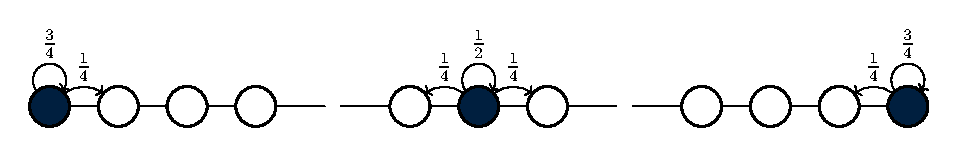
\includegraphics[width=0.95\linewidth]{figures/appendix/lazzy_symmetry_random_walk.pdf}
    \caption{Cases of lazy random walk. The circles represent the sites of the lattice $\{y_1, y_2, \cdots, y_n\}$, while the black circle stands for the starting site $y_i$, and the numbers over arrows are transition probability.}
    \label{fig: lazy random walk}
\end{figure}

The function $L$ in Table \ref{table: transition table of teto} is the transition function of 1D symmetry lazy random walk (SLRW). 
In 1D-SLRW, a point located at a site $y_i$ has a probability of $0.25$  moving to one of its neighboring sites $y_{i-1}$ or $y_{i+1}$, and it has a probability of $0.5$ staying in place. If the origin site is on the ends of the lattice, it has a probability of $0.75$ staying in place and has a probability of $0.25$ moving around. The cases of 1D-SLRW is shown in Fig.~\ref{fig: lazy random walk}, which is expressed by 
\begin{equation}
\label{eq: lazy random walk L}
L\left(y_i\right)=
\begin{cases}
\frac{3}{4} y_1+\frac{1}{4} y_2, &i=1 \\
\frac{1}{4} y_{i-1}+\frac{1}{2} y_i+\frac{1}{4} y_{i+1}, &1<i<N \\
\frac{3}{4} y_N+\frac{1}{4} y_{N-1}, &i=N
\end{cases}.
% \left\{\begin{array}{l}
% \end{array}\right.
\end{equation}


Table \ref{table: transition table of teto} shows that $\Tcouple$ could be considered as two independent 1D-SLRW except for the cases that $\abs{i-j}\leq 1$. It suggests that the result of evolution could be separated into two parts, the 1D-SLRW part and the remind part
\begin{equation}
    \alpha_{\{\gamma_i \gamma_j\}, 2t+1} = \alpl + \alpr.
\end{equation}
Here, we denote $\alpha_{S, d}$ as $\alpha_{\{\gamma_i \gamma_j\}, 2t+1}$ because the $S$ is restricted to 1-RDM and the number of layers is odd. The SLRW part $\alpl$ is the value of $\alpha_{\{\gamma_i \gamma_j\}, 2t+1}$ if the state transition follow the 1D-SLRW in all sites $y_i y_j$,
\begin{equation}
\label{eq: alpl main expr}
    \alpl = \sum_k \frac{\partial^2}{\partial y_k^2} L^t(y_i)L^t(y_j),
\end{equation}
where $L^t(y_i)$ is the $t$-times composition of $L$, $L^t(y_i) = L\circ \cdots \circ L (y_i)$. The deduction of Eq.~\ref{eq: alpl main expr} is shown in Appendix \ref{sec: mapping the action of tensors to random walk}. And we simplified the expression to a more analytically tractable form. 
\begin{theorem}
    \label{theorem: order of alpha l}
    Given $t = o(n^2) $, the $\alpl$ could be estimated by the following formula
    \begin{equation}
        3\alpl = \frac{1}{\sqrt{2\pi t}} (e^{-\frac{a^2}{2t}}+ e^{-\frac{b^2}{2t}}) + \frac{2}{\sqrt{2\pi t}}(e^{-\frac{a^2+n(n/2-a)}{2t}}+ e^{-\frac{b^2+n(n/2-b)}{2t}}) + \mathcal{O}\left(e^{-\frac{\pi^2}{2}t}\right),
    \end{equation}
    where $a$ is $|i-j|$ and $b$ is $i+j-1$. The notation $o(n^2)$ denotes a function that grows slower than $n^2$ as $n$ approaches infinity. 
\end{theorem}
\textcolor{cyan}{explain why we do not care $t=\Omega(n^2)$}

Here, we estimate the order of $\alpl$ first. Then we show that the $\alpl$ is 
the dominant part that determined the order of $\alpha_{\{\gamma_i \gamma_j\}, 2t+1}$ because the $\alpr$ is negative and greater than $-c \alpl$ with a constant $c<1$. 
Since $a<b$ and $a^2 < a^2+2N(N-a)$, the order of alpha is determined by the dominant part $ \frac{1}{\sqrt{2\pi t}} e^{-\frac{a^2}{2t}}$. The order of the term $ \frac{1}{\sqrt{2\pi t}} e^{-\frac{a^2}{2t}}$ depends on the order of $a$. This term scales $\frac{1}{\mathrm{poly}(n)}$ if and only if $\frac{a^2}{2t} = \mathcal{O}(\log(n))$, which equivalent to $t = \mathcal{O}(\frac{a^2}{\log(n)})$. We leave the proof in Appendix \ref{sec: estimate the order of alpl}


Denote the output of the whole tensor network as 
\begin{equation}
    \left(\Tcouple\right)^t ( y_i y_j) = \sum_{l,k} \mathrm{Prob}(S_t = y_l y_k \mid S_0 = y_i y_j) y_l y_k, 
\end{equation}
where $\mathrm{Prob}(S_t = y_l y_k \mid S_0 = y_i y_j)$ is the probability of traveling from the starting point $y_iy_j$ to end point $y_ly_k$ in $t$ steps transition. We observe that the transition probability $\mathrm{Prob}(S_t = y_k^2 \mid S_0 = y_i y_j)$ is less than the transition probability of SLRW part $\frac{\partial^2}{\partial y_k^2} L^t(y_i)L^t(y_j) $, and it is opposite in the rest part. With this assumption, we bound $\alpr$ with $\alpl$:
\begin{theorem}
\label{theorem: relation between alpha L and alpha R}
    Assume that $\mathrm{Prob}(S_t = y_k^2\mid S_0 = y_i y_j) < \frac{\partial^2}{\partial y_k^2} L^t(y_i)L^t(y_j) $ for all $k$, and $\mathrm{Prob}(S_t = y_l y_k \mid S_0 = y_i y_j) > \frac{\partial^2}{\partial y_k^2} L^t(y_i)L^t(y_j)$ for $l\neq k$. Then, $\alpr$ satisfies the following property
    \begin{equation}
        -\alpr \leq \frac{25}{72} \max_{k \geq 0}\left\{ \alpha_{\{\gamma_i\gamma_j\}, 2t-2k+1} \right\}
    \end{equation}
\end{theorem}





\subsection{Fitting required depth for k-RDM}
Suppose the elements of $S$ are $i_1, i_2, \cdots, i_{|S|}$ which satisfies $i_1 < i_2 < \cdots < i_{|S|}$.
Define the distance of $|S|$ as
\begin{equation}
    d(S) := \max(|i_{2j-1}-i_{2j}|\mid j \in \{1, 2, \cdots \frac{|S|}{2}\}).
\end{equation}
The number $\frac{|S|}{2}$ is an integer because 
\begin{equation}
    \alpha_{S', d} =0
    \label{eq: zz anonymous 8}
\end{equation}
when $|S'|$ is an odd number~\cite{wan2022matchgate}. Intuitively, Eq.~\eqref{eq: zz anonymous 8} is true because we measure the state on computational basis. The computational basis can only consist of operators $\gamma_S$. Thus, we only care about the set $S$ with even cardinal number.
Then, we have the following theorem:
\begin{theorem}
The expectation value of $\tr(\rho \gamma_S)$ can be obtained by using $\polylog(n)$-layers matchgate circuit within the Fermionic classical shadows protocol, when the distance of $S$ is $\mathcal{O}(\log n)$ and the cardinal number $|S|$ is a constant $2c$.
    % It only needs $\polylog(n)$-layers matchgate circuit to get the expectation value of $\tr(\rho \gamma_S)$ within the Fermionic classical shadows protocol.  
\end{theorem}


\section{Numerical simulation}

% \section{Appendix}

\bibliographystyle{unsrt}
\bibliography{ref}
\appendix

\section{Proof of Lemma \ref{lemma 1}}
\begin{proof}
The state $\ket{b}= \ket{b_1b_2\cdots b_n}$ could be denoted as $\prod X_{b_i} \ket{0}$. 
Since Pauli-$X$ is in the matchgate group, we can absorb the $\prod X_{b_i}$ into the matchgates $U_{Q_d}$ in the expression of shadow channel
\begin{align}
\mathcal{M}_d(\gamma_S) &= \int \dd U_{Q_d}\sum_{b\in\{0,1\}^n}\bra{b}U_{Q_d}\gamma_S U_{Q_d}^\dagger \ket{b} U_{Q_d}^\dagger \ket{b}\bra{b}U_{Q_d}\\
&= 2^n\int \dd U_{Q_d} \bra{0}U_{Q_d}\gamma_S U_{Q_d}^\dagger \ket{0} U_{Q_d}^\dagger \ket{0}\bra{0}U_{Q_d}.
\end{align}
%By a similar technique as Lemma 12 of Ref. \cite{bertoni2022shallow}, we see that 
If $S'$ is not equal to $ S$ and the layer number $d$ is not equal to zero, 
then there exists a permutation matrix $Q$ such that
% \begin{align}
% Q|_{S,S} = \mathbbm{1}, \quad Q|_{S',S'} = -\mathbbm{1},
% \end{align}
% and hence
\begin{align}
\quad [\gamma_{S}, U_{Q}] = 0, \quad \{\gamma_{S'}, U_{Q'}\} = 0. 
\end{align}
It implies
\begin{align}
\frac{1}{2^n}\tr{\gamma_{S'} \mathcal{M}_d(\gamma_S)} &= 
\int \dd U_{Q_d} \bra{0} U_{Q_d} \gamma_S U_{Q_d}^\dagger \ket{0}\bra{0}U_Q \gamma_{S'} U_{Q_d}^\dagger\ket{0}\\
&=\int \dd U_{Q_d} \bra{0}U_{Q_d} U_{Q'_d} \gamma_S U_{Q'_d}^\dagger U_{Q_d}^\dagger\ket{0}\bra{0}U_{Q_d} U_{Q'_d}\gamma_{S'} U_{Q'_d}^\dagger U_{Q_d}^\dagger\ket{0}\\
&= -\int \dd U_{Q_d} \bra{0}U_{Q_d} \gamma_S U_{Q_d}^\dagger\ket{0}\bra{0}U_{Q_d} \gamma_{S'} U_{Q_d}^\dagger\ket{0}.
\end{align}
Hence $\mathcal{M}_d (\gamma_S) = \alpha_{s,d} \gamma_S$.
\end{proof}


\section{Proof of Lemma \ref{lemma 2}}
\begin{proof}
Let the estimator of the observable $\gamma_S$ be $v$.
\begin{align}
\Var[v] &\leq \mean[\abs{v}^2]\\
&= \int \dd U_{Q_d}
 \mean_{\rho}\left[\sum_b \bra{b}U_{Q_d} \rho U_{Q_d}^\dagger\ket{b} \abs{\bra{b}U_{Q_d} \mathcal{M}_d^{-1} (\gamma_S) U_{Q_d}^\dagger \ket{b}}^2\right]\\
 &=2^{-n}\int  \dd U_{Q_d} \sum_b \abs{\bra{b}U_{Q_d} \mathcal{M}_d^{-1} (\gamma_S) U_{Q_d}^\dagger\ket{b}}^2\\
 &=\frac{1}{\abs{\alpha_{S,d}}^2} \int \bra{0}U_{Q_d} \gamma_S U_{Q_d}^\dagger\ket{0}\bra{0}U_{Q_d} \gamma_S^\dagger U_{Q_d}^\dagger\ket{0}\\
 &=\frac{1}{\alpha_{S,d}}.
 \end{align}


\section{Proof of Lemma \ref{lemma 3}}
\label{appendix 3}
 In this section, we represent the variance of Fermionic classical shadow in the form of a tensor network.
The variance is bounded by $1/\alpha_{S,d}$, where
\begin{align}
    % \label{eq: appendix alpha}
    \alpha_{S,d} =& \int_{Q\sim O_d } \dd \mu(Q) \abs{\bra{0} U_Q \gamma_S U_Q^\dagger \ket{0}}^2 \\
    =& \int_{Q\sim O_d } \dd \mu(Q) \bra{0} U_Q \gamma_S U_Q^\dagger \ket{0}\bra{0} U_Q \gamma_S^\dagger U_Q^\dagger \ket{0}.
\end{align}
The subscript $d$ denotes the layer number of the matchgate circuit. 
The expression could be simplified by substituting the relationship between $\gamma_S^\dagger$ and $\gamma_S$, which is 
\begin{equation}
    \gamma_S^\dagger = (-1)^{\frac{|S|(|S|-1)}{2}}\gamma_S.
\end{equation}
The relation is true because of the anti-commutation relation of Majorana operators $\{\gamma_i, \gamma_j\} = 2\delta_{ij}$. The anti-commutation relation produces a coefficient of $(-1)^{|S|-1}$ when $\gamma_{l_1}$ is moved to the first place. 
Then, the $\gamma_S^\dagger$ could be calculated by
\begin{align}
    \gamma_S^\dagger=& (-1)^{|S|-1}\gamma_{l_1}\gamma_{l_{|S|}}\gamma_{l_{|S|-1}}\cdots \gamma_{l_2}\\
    =& (-1)^{|S|-1 + |S|-2} \gamma_{l_1}\gamma_{l_2}\gamma_{l_{|S|}}\gamma_{l_{|S|-1}}\cdots \gamma_{l_3}\\
    \label{eq: gammaSgamma}
    =& (-1)^{\frac{|S|(|S|-1)}{2}}\gamma_S.
\end{align}
By substituting Eq.~\eqref{eq: gammaSgamma}, the $\alpha_{S, d}$ could be expressed as  
\begin{align}
    \alpha_{S,d} =& (-1)^{\frac{|S|(|S|-1)}{2}} \int_{Q \sim O_d} \dd\mu(Q) 
    \bra{0}U_Q \gamma_SU_Q^\dagger\ket{0}^2\\
    =& (-1)^{\frac{|S|(|S|-1)}{2}} \int_{Q \sim O_d} \dd\mu(Q) 
    \tr(U_Q \gamma_SU_Q^\dagger\ket{0} \bra{0} )^2\\
    =& (-1)^{\frac{|S|(|S|-1)}{2}} 2^{2n} \int_{Q \sim O_d} \dd\mu(Q) 
    \supbra{0,0} \mathcal{U}_Q\otimes\mathcal{U}_Q \supket{\gamma_S,\gamma_S} \\
    =& (-1)^{\frac{|S|(|S|-1)}{2}} 2^{2n}  \supbra{0,0}  \int_{Q \sim O_d}\dd\mu(Q) \mathcal{U}_Q^{\otimes 2} \supket{\gamma_S,\gamma_S}.
\end{align}
In the third line, we rewrite the formula regarding super vectors and super operators. The integral of the form $\int \dd \mu(Q) \mathcal{U}_Q^{\otimes k}$ is known as the twirling. Sometimes we will use the terminology \textit{twirling} for simplification.



The $d$-layers matchgate circuit is composed of interweaving stacking two-qubits matchgates. Thus, to calculate the integral $\int_{Q \sim O_d} \dd\mu(Q) \mathcal{U}_Q^{\otimes 2}$, we could independently calculate the integral of each $2$ qubits matchgates. The result of the integral of the $2$ qubits matchgates is given by Lemma \ref{lem:threemomentsMatchgate}
\begin{align}
\label{eq: integral of the 2 qubits matchgates}
    \int_{Q\sim M_2} \dd\mu(Q)\mathcal{U}_Q^{\otimes 2} =& \supketbra{\gamma_\emptyset}{\gamma_\emptyset}
    + \frac{1}{4} \sum_{i,j} \supketbra{\gamma_i}{\gamma_j}\\
    &+ \frac{1}{6}\sum_{\substack{i_1\neq i_2 \\ j_1\neq j_2}}\supketbra{\gamma_{i_1}\gamma_{i_2}}{\gamma_{j_1}\gamma_{j_2}} \\
    &+ \frac{1}{4}
    \sum_{\substack{i_1\neq i_2, j_1 \neq j_2 \\ 
        i_1\neq i_3, j_1 \neq j_3 \\
        i_2\neq i_3, j_2 \neq j_3} 
    }
    \supketbra{\gamma_{i_1}\gamma_{i_2}\gamma_{i_3}}{\gamma_{j_1}\gamma_{j_2}\gamma_{j_3}}\\
    &+ \supketbra{\gamma_1\gamma_2\gamma_3\gamma_4}{\gamma_1\gamma_2\gamma_3\gamma_4},
\end{align}
where $i$, $j$ are index ranged from $1$ to $4$. 



To calculate the interweaving stacking of two-qubits matchgates, we represent the super vectors $\supket{\gamma_S}$ using the Pauli basis through the Jordan-Wigner transformation. Due to the transformation, the $\gamma_S$ is corresponded to a Pauli basis with a phase $\pm \ii^{\floor{|S|/2}}$. Thus, the super vector $\supket{\gamma_S, \gamma_S}$ could be represented as 
\begin{equation}
    \supket{\gamma_S, \gamma_S} = (-1)^{\floor{\frac{|S|}{2}}} \supket{P^{S}, P^{S}},
\end{equation}
 where $P^{S}$ is the Pauli operator that corresponding to the $\gamma_S$.
Therefore, due to the Lemma \ref{lemma: The net phase of alpha is 1}, the net phase of the $\alpha_{S,d}$ is $1$. 

We also represent the integral of the $2$ qubits matchgates with Pauli basis by applying the Jordan-Wigner transformation to Eq.~\eqref{eq: integral of the 2 qubits matchgates}. Denote the twirling as a $4$-bond tensor as the following rule,
\begin{equation}
\label{eq: definition of T}
    T^{\sigma_1, \sigma_2}_{~~\sigma_3, \sigma_4} = \supbra{\sigma_1, \sigma_2}\supbra{\sigma_1, \sigma_2}\int_{Q\sim M_2} \dd\mu(Q)\mathcal{U}_Q^{\otimes 2} \supket{\sigma_3, \sigma_4}\supket{\sigma_3, \sigma_4},
\end{equation}
where $\sigma_1, \sigma_2, \sigma_3, \sigma_4$ are two-qubits Pauli operators. The concrete elements of the tensor $T$ is shown in the Table \ref{table: the 16x16 matrix of T}. For example, due to Eq.~\eqref{eq: integral of the 2 qubits matchgates} and Eq.~\eqref{eq: definition of T}, $T^{XY}_{~~YZ}$ is equal to $\frac{1}{6}$. 

% The twirling of a $d$-layer matchgate circuit can be represented as a tensor network composed of $T$ tensors, as illustrated in Fig.~\ref{fig:TNcoefRep}. \textcolor{cyan}{polish the figure}

To build the tensor network, we will define some notation. Let $T^{(o)}$ represent the odd-layer of T gates, and $T^{(e)}$ represent the even-layer of $T$ gates, which are shown in the following circuits.
\begin{figure}[H]
    \centering
    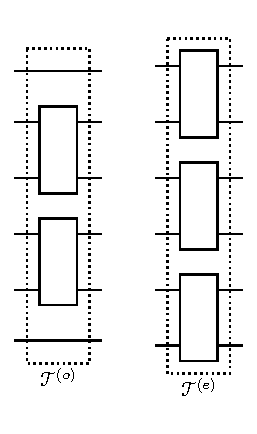
\includegraphics[width=0.22\linewidth]{figures/appendix/Todd_Teven.pdf}
    % \caption{Caption}
    % \label{fig:enter-label}
\end{figure}
The whole tensor network $\Twhole$ could be expressed by alternately apply $T^{(o)}$ and $T^{(e)}$ gates, 
\begin{equation}
\Twhole \left(t, b_1, b_2\right)=T^{(o)^{b_2}}\left(\prod_{i=0}^{t} T^{(e)} T^{(o)}\right) T^{(e)^{b_1}}, 
\end{equation}
where $b_1, b_2 \in\{0,1\}$, $t+b_1+b_2$ stands for the number of layers.


The calculation of $\alpha_{S,d}$ could be represented by the tensor network contraction.
Notice the matrix identity 
\begin{equation}
    \ketbra{0} = \frac{1}{2^n} \sum_{\Lambda\subset [2n]} \prod_{i \in \Lambda} Z_i,
\end{equation}
where $Z_i$ denotes the application of the Pauli Z operator to the $i$-th qubit.
Specially, let $\prod_{i \in \emptyset} Z_i = \mathbb{I}_n$. Then, the super vector of $\supket{0,0}$ could be expressed as
\begin{equation}
\label{eq: zz anonymous 6}
    \supket{0,0} = \frac{1}{2^{2n}} \sum_{\Lambda, \Lambda' \subset [2n]}  \supket{\prod_{i \in \Lambda }  Z_i, \prod_{j \in \Lambda'} Z_j}.
\end{equation}
By transforming all the super vectors and the super operators in the Pauli basis, 
the evolution of $\mathcal{U}_Q \supket{\gamma_S}$ could be equivalently expressed by 
\begin{equation}
\label{eq: transfer evolution of U to tensor}
    \int \dd\mu(Q) \mathcal{U}_Q^{\otimes 2} \supket{\gamma_S,\gamma_S} = \Twhole \supket{P^S}.
\end{equation}
In the equation, for simplicity, we slightly abuse the notation $\supket{P^S}$ to represent the tensor of Pauli basis $\supket{P^S, P^S}$. Formally, $\supket{P^S}$ is the tensor $\delta_{S}^{R}$, where $\delta_{S}^{R}=1$ if and only if $R=S$, otherwise, $\delta_{S}^{R}=0$. In this representation, The tensor contraction $\Twhole(t, b_1, b_2) P^S$ is equivalent to the evolution $\int \dd\mu(Q) \mathcal{U}_Q^{\otimes 2} \supket{\gamma_S,\gamma_S}$. Thus, the calculation of $\alpha_{S,d}$ could be expressed as the tensor network contraction, as illustrated in Fig.~\ref{fig:TNcoefRep}. \textcolor{cyan}{polish the figure}







\begin{lemma}[Theorem 1 in \cite{wan2022matchgate}]
    Let $Q$ be a matrix uniformly randomly sampled from orthogonal group $\mathcal{O}(n)$, then
\begin{align}
& \int_{Q\sim M_n} \dd\mu(Q) \mathcal{U}_Q = \supket{\mathbb{I}}\supbra{\mathbb{I}}\\
& \int_{Q\sim M_n} \dd\mu(Q)\mathcal{U}_Q^{\otimes 2} = \sum_{k=0}^{2n}\supket{\mathcal{R}_k^{(2)}}\supbra{\mathcal{R}_k^{(2)}}\\
& \int_{Q\sim M_n} \dd\mu(Q)\mathcal{U}_Q^{\otimes 3} = \sum_{
\substack{
k_1,k_2,k_3\geq 0\\
k_1 + k_2 + k_3\leq 2n
}
}\supket{\mathcal{R}_{k_1,k_2,k_3}^{(3)}}\supbra{\mathcal{R}_{k_1,k_2,k_3}^{(3)}}.
\end{align}
where
\begin{align}
    &\supket{\mathcal{R}_k^{(2)}} = { 2n\choose k}^{-1/2} \sum_{S\subseteq [2n],|S|=k}\supket{\gamma_S}\supket{\gamma_S}\\
    &\supket{\mathcal{R}_k^{(3)}} = {2n \choose k_1,k_2,k_3,2n-k_1-k_2-k_3}^{-1/2} \sum_{
    \substack{
 S_1, S_2, S_3\subseteq [2n] disjoint\\
 \abs{S_j}=k_j,1\leq j\leq 3
    }
    } \supket{\gamma_{S_1}\gamma_{S_2}}
    \supket{\gamma_{S_2}\gamma_{S_3}}
    \supket{\gamma_{S_3}\gamma_{S_1}}
\label{eq:third_moment}
\end{align}
\label{lem:threemomentsMatchgate}
\end{lemma}

\begin{lemma}
\label{lemma: The net phase of alpha is 1}
    The net phase of $\alpha_{S,d}$ is $1$.
\end{lemma}
\begin{proof}
    The net phase of $\alpha_{S,d}$ is $1$ is $(-1)^{\frac{|S|(|S|-1)}{2}} (-1)^{\floor{|S|/2}}$. We categorize the discussion of the parity of $|S|$.
    \begin{enumerate}
        \item \textbf{$|S|$ is an odd number.} Let $|S| = 2q+1$, $ q\in \mathbb{N}$, $q\geq 0$. And then
        \begin{equation}
            (-1)^{\frac{|S|(|S|-1)}{2}} (-1)^{\floor{|S|/2}} = (-1)^{q(2q+1)+q} = 1.
        \end{equation}
        \item \textbf{$|S|$ is an even number.} Let $|S| = 2q$, $ q\in \mathbb{N}$, $q\geq 0$. And then
        \begin{equation}
            (-1)^{\frac{|S|(|S|-1)}{2}} (-1)^{\floor{|S|/2}} = (-1)^{(2q-1)q+q} = 1.
        \end{equation}
    \end{enumerate}
\end{proof}

\begin{table}
\centering
\begin{tabular}{|c|c|c|c|c|c|c|c|c|c|c|c|c|c|c|c|c|}
	\hline
	T  &II &IX &IY &IZ &XI &XX &XY &XZ &YI &YX &YY &YZ &ZI &ZX &ZY &ZZ \\ \hline
    II & 1 &   &   &   &   &   &   &   &   &   &   &   &   &   &   &   \\ \hline
    IX &   &1/4&1/4&   &   &   &   &1/4&   &   &   &1/4&   &   &   &   \\ \hline
    IY &   &1/4&1/4&   &   &   &   &1/4&   &   &   &1/4&   &   &   &   \\ \hline
    IZ &   &   &   &1/6&   &1/6&1/6&   &   &1/6&1/6&   &1/6&   &   &   \\ \hline
    XI &   &   &   &   &1/4&   &   &   &1/4&   &   &   &   &1/4&1/4&   \\ \hline
    XX &   &   &   &1/6&   &1/6&1/6&   &   &1/6&1/6&   &1/6&   &   &   \\ \hline
    XY &   &   &   &1/6&   &1/6&1/6&   &   &1/6&1/6&   &1/6&   &   &   \\ \hline
    XZ &   &1/4&1/4&   &   &   &   &1/4&   &   &   &1/4&   &   &   &   \\ \hline
    YI &   &   &   &   &1/4&   &   &   &1/4&   &   &   &   &1/4&1/4&   \\ \hline
    YX &   &   &   &1/6&   &1/6&1/6&   &   &1/6&1/6&   &1/6&   &   &   \\ \hline
    YY &   &   &   &1/6&   &1/6&1/6&   &   &1/6&1/6&   &1/6&   &   &   \\ \hline
    YZ &   &1/4&1/4&   &   &   &   &1/4&   &   &   &1/4&   &   &   &   \\ \hline
    ZI &   &   &   &1/6&   &1/6&1/6&   &   &1/6&1/6&   &1/6&   &   &   \\ \hline
    ZX &   &   &   &   &1/4&   &   &   &1/4&   &   &   &   &1/4&1/4&   \\ \hline
    ZY &   &   &   &   &1/4&   &   &   &1/4&   &   &   &   &1/4&1/4&   \\ \hline
    ZZ &   &   &   &   &   &   &   &   &   &   &   &   &   &   &   & 1 \\ \hline
\end{tabular}
\caption{Values of tensor $T$. The head of columns represents the input of $T$ while the head of rows represents the output of $T$. For example, the value in row `XY' and column `YZ' represent the value $T^{XY}_{~~YZ}$.  The blank space of the table stands for $0$.    }
\label{table: the 16x16 matrix of T}
\end{table}
\end{proof}


\section{Mapping the action of tensors to random walk}
\label{sec: Mapping the action of tensors to random walk}
\subsection{Reduce the calculation to polynomial space}
\begin{figure}
    \centering
    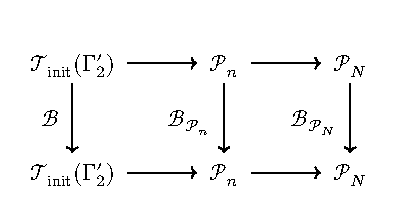
\includegraphics[width=0.8\linewidth]{figures/appendix/commute_diagram.pdf}
    \caption{The diagram shows how we simplify the calculation step by step. The horizontal arrows point from a high-dimensional space to a relatively low-dimensional space. The vertical arrows stand for the corresponding operators of $\Twhole(t,b_1, b_2)$ in different representations. Finally, we reduce it to the $N$-elementary polynomial of the $2$nd degree polynomial space.}
    \label{diagram: commute diagram}
\end{figure}

% We use polynomial space to represent $\Twhole$ because polynomial space obtains the properties we need, like multiplication and addition that we will use later.
We represent $\Twhole$ using polynomial space because it provides the essential properties we require, such as multiplication and addition, which will be important for our later work. 

Notice that the space $V_P$ is isometric to the $n$-elementary polynomial of the $2$nd degree polynomial space $\mathcal{P}_n$. The isometric could be constructed by the following
\begin{equation}
    \begin{aligned}
        \phi : V_P &\to \mathcal{P}_n \\
        \supket{M_i(\prod Z_k)M_j} &\mapsto x_i x_j \\
        \supket{Z_i} &\mapsto x_i^2.
    \end{aligned}
\end{equation}
The linear map $\phi$ is a homomorphism with inverse, which means it is an isometric between $V_P$ and $\mathcal{P}_n$. The equivalent representation of $\Twhole$ could be constructed by
\begin{equation}
    \Twhole_{\mathcal{P}_n}(t) (\cdot) := \phi \circ \Twhole(t,1,0) \circ \phi^{-1} (\cdot).
\end{equation}
% Thus, we build the equivalent representation $\mathcal{P}_n$ with group action $\Twhole_{\mathcal{P}_n}(t)$.
% which is shown in the second loop in the Fig.~\ref{diagram: commute diagram}. 
We could also transfer the input of $\Twhole$ to space $\mathcal{P}_n$,
\begin{equation}
    \gamma_{ij} \longrightarrow \supket{M_i(\prod Z_k)M_j} \xrightarrow{~~\phi~~} x_i x_j.
\end{equation}
Thus, the action of $d$-layer matchgate circuit on the $\gamma_{ij}$ is equivalent to the action of $\Twhole_{\mathcal{P}_n}(t)$ on the term $x_i x_j$. 
Due to Lemma \ref{lemma: reduce Pn to PN}, the action could be further simplified by finding a sub-representation $\mathcal{P}_N$ of representation $\mathcal{P}_n$, where $N$ equals to $\frac{n}{2}$. Recall that $n$ is an even number so $N$ is an integer. 

% By reducing the representation to the polynomial space $\mathcal{P}_N$, some patterns are revealed so that we could analysis it. 
Certain hidden patterns are revealed by reducing the representation to the polynomial space $\mathcal{P}_N$. Most of the main results are been proved in the $\mathcal{P}_N$. 
% Most of the main results are proved on the 


\begin{lemma}
    \label{lemma: reduce Pn to PN}
    The space $\mathcal{P}_N$ isometric to a sub-representation of $\mathcal{P}_n$.
\end{lemma}
\begin{proof}
    Define the map $\phi$ as
    \begin{equation}
        \begin{aligned}
            \phi : \mathcal{P}_N &\to \mathcal{P}_n \\
              y_i^2 &\mapsto x_{2i-1}^2+4 x_{2i-1} x_{2i}+x_{2i}^2\\
           y_i y_j &\mapsto  \left(x_{2i-1}+x_{2i}\right)\left(x_{2j-1}+x_{2j}\right).
        \end{aligned}
    \end{equation}
    We define the  $\phi$ as a linear function so that the definition of mapping on a basis induces the mapping on any element of the space
    \begin{equation}
        \phi(\sum \xi_{ij}y_i y_j) = \sum \xi_{ij}\phi(y_i y_j).
    \end{equation}
    Thus, the space $\phi(\mathcal{P}_N)$ is a linear subspace of $\mathcal{P}_n$. Because $\phi$ is an injection, there is a map $\phi': \mathcal{P}_n \to \mathcal{P}_N$ such that $\phi' \circ\phi$ is identity. 
    Define the group action $\Twhole_{\mathcal{P}_N}$ as 
    \begin{equation}
        \Twhole_{\mathcal{P}_N}(y_i y_j) := \phi' \circ \Twhole_{\mathcal{P}_n}\circ \phi(y_i y_j).
    \end{equation}
    Based on the definition of representation, we know that the space $\mathcal{P}_N$ with the group action $\Twhole_{\mathcal{P}_N}$ is a representation. 
    
    The next step is to show that such a representation $\Twhole_{\mathcal{P}_N}$ does not lose information. Formally, we need to prove that the representation $\mathcal{P}_n$ could be reduced to a sub-representation isometrics to $\mathcal{P}_N$. Naturally, we will consider whether the subspace $\phi(\mathcal{P}_N) $ will constitute a sub-representation. If it is true, the proof is done because $\phi(\mathcal{P}_N) \simeq \mathcal{P}_N$.

    By the definition of sub-representation, we need to prove
    \begin{equation}
    \label{eq: PN is a sub representation}
        \Twhole_{\mathcal{P}_n}(t)(\phi(\mathcal{P}_N)) \subset \phi(\mathcal{P}_N), ~~\forall t .
    \end{equation}
    The readers may recall that the formal representation is $T^{(e)}_{\mathcal{P}_n} \phi(\mathcal{P}_N)$ rather than $\phi(\mathcal{P}_N)$. Here, we remove the ambiguity by proving $T^{(e)}_{\mathcal{P}_n} \phi(\mathcal{P}_N) = \phi(\mathcal{P}_N)$. 
    By expanding the definition of $T^{(e)}_{\mathcal{P}_n}$, we could get the calculation of $T^{(e)}_{\mathcal{P}_n} \phi(y_i y_j)$ backs to the space $V_P$. Then, we will find that $T^{(e)}_{\mathcal{P}_n} \phi(y_i y_j) = \phi(y_i y_j)$ from the Table~\ref{table: the 16x16 matrix of T}. Thus, we have $T^{(e)}_{\mathcal{P}_n} \phi(\mathcal{P}_N) = \phi(\mathcal{P}_N)$.
 
    The statement \eqref{eq: PN is a sub representation} will be proved by induction.
    
     When $t=0$, $T^{(e)}_{\mathcal{P}_n} \phi(\mathcal{P}_N)\subset \phi(\mathcal{P}_N)$ is true.
     Suppose the statement is true for $t^*$, then we have
    \begin{equation}
        \Twhole_{\mathcal{P}_n}(t^*)(\phi(y_iy_j)) = \sum \xi_{lm} \phi(y_ly_m).
    \end{equation}
    And then
    \begin{align}
        \Twhole_{\mathcal{P}_n}(t^*+1)(\phi(y_i y_j)) =& 
        T^{(e)}_{\mathcal{P}_n}T^{(o)}_{\mathcal{P}_n} (\sum \xi_{lm} \phi(y_ly_m)) \\
        \label{eq: zz anonymous 2}
        =& \sum \xi_{lm} \delta_{lm}T^{(e)}_{\mathcal{P}_n}T^{(o)}_{\mathcal{P}_n} ( x_{2i-1}^2+4 x_{2i-1} x_{2i}+x_{2i}^2) \\
        \label{eq: zz anonymous 3}
        & + \sum \xi_{lm} (1-\delta_{lm})T^{(e)}_{\mathcal{P}_n}T^{(o)}_{\mathcal{P}_n}\left(\left(x_{2 i-1}+x_{2 i}\right)\left(x_{2 j-1}+x_{2 j}\right)\right)
    \end{align}
    We will prove Eq.~\eqref{eq: zz anonymous 2} is in the space $\phi(\mathcal{P}_N)$, while the same result of Eq.~\eqref{eq: zz anonymous 3} can be proved by the same method. Now, we will directly calculate this expression
    \begin{equation}
    \begin{aligned}
        \label{eq: zz anonymous 4}
        &T^{(e)}_{\mathcal{P}_n}T^{(o)}_{\mathcal{P}_n} ( x_{2i-1}^2+4 x_{2i-1} x_{2i}+x_{2i}^2) \\
        =& T^{(e)}_{\mathcal{P}_n}(\frac{1}{6}x_{2i-2}^2 + \frac{2}{3} x_{2i-2}x_{2i-1} + x_{2i-2}x_{2i}+x_{2i-2}x_{2i+1} \\
        &+\frac{1}{6} x_{2i-1}^2 + x_{2i-1}x_{2i} + x_{2i-1}x_{2i+1}  \\
        &+\frac{1}{6} x_{2i}^2 + \frac{2}{3} x_{2i}x_{2i+1} + \frac{1}{6}x_{2i+1}^2  )\\
        =& \frac{1}{36}x_{2i-3}^2 + \frac{1}{9} x_{2i-3}x_{2i-2} +\frac{5}{12} x_{2i-3}x_{2i-1}+ \frac{5}{12} x_{2i-3}x_{2i}  + \frac{1}{4} x_{2i-3}x_{2i+1} + \frac{1}{4} x_{2i-3}x_{2i+2}  \\
        &+ \frac{1}{36}x_{2i-2}^2 + \frac{5}{12} x_{2i-2}x_{2i-1}+ \frac{5}{12} x_{2i-2}x_{2i}  + \frac{1}{4} x_{2i-2}x_{2i+1} + \frac{1}{4} x_{2i-2}x_{2i+2}  \\
        &+ \frac{2}{9}x_{2i-1}^2 + \frac{8}{9} x_{2i-1}x_{2i} + \frac{5}{12} x_{2i-1}x_{2i+1} + \frac{5}{12} x_{2i-1}x_{2i+2}\\
        & + \frac{2}{9}x_{2i}^2 + \frac{5}{12} x_{2i}x_{2i+1} + \frac{5}{12} x_{2i}x_{2i+2}\\
        & + \frac{1}{36}x_{2i+1}^2  + \frac{1}{9} x_{2i+1}x_{2i+2}\\
        & + \frac{1}{36}x_{2i+2}^2 \\
        % =& \frac{1}{6} y_{i-1}^2 + \frac{5}{3} y_{i-1}y_{i} + y_{i-1}y_{i+1} + \frac{4}{3} y_{i}^2 + \frac{5}{3} y_{i-1}y_{i+1}  + \frac{1}{6} y_{i+1}^2
    \end{aligned}
    \end{equation}
    The result expression is in $\phi(\mathcal{P}_N)$ because we could find a polynomial $y$ in $\mathcal{P}_N$ such that $\phi(y)$ equals the result expression,
    \begin{align}
        y =& \frac{1}{6} y_{i-1}^2 + \frac{5}{3} y_{i-1}y_{i} + y_{i-1}y_{i+1} + \frac{4}{3} y_{i}^2 + \frac{5}{3} y_{i-1}y_{i+1}  + \frac{1}{6} y_{i+1}^2 \\
        \phi(y) =& T^{(e)}_{\mathcal{P}_n}T^{(o)}_{\mathcal{P}_n} ( x_{2i-1}^2+4 x_{2i-1} x_{2i}+x_{2i}^2)
    \end{align}
    Thus, we get that 
    \begin{equation}
        T^{(e)}_{\mathcal{P}_n}T^{(o)}_{\mathcal{P}_n} ( x_{2i-1}^2+4 x_{2i-1} x_{2i}+x_{2i}^2) \subset \phi(\mathcal{P}_N).
    \end{equation}
    Thus, Eq.~\eqref{eq: zz anonymous 4} is contained in the space $\phi(\mathcal{P}_N)$, which completes the proof.
\end{proof}


% By studying the property of $\Twhole$, we could find a sub-representation of $\mathcal{P}_n$. Firstly, we transfer the input of $\Twhole$ to space $\mathcal{P}_n$,
% \begin{equation}
%     \gamma_{ij} \longrightarrow \supket{M_i(\prod Z_k)M_j} \xrightarrow{~~\phi~~} x_i x_j.
% \end{equation}
% With Lemma we prove that the output of $\Twhole_{\mathcal{P}_n}(t)$ obtains the 

\subsection{Mapping the spread of polynomials to random walk}
\label{sec: mapping the action of tensors to random walk}

\newcommand{\teto}{T^{(e)}_{\mathcal{P}_N}T^{(o)}_{\mathcal{P}_N}}
The action of layers is the lazy-symmetry random walk on a 2D square lattice in most sites. To illustrate this point, we will begin with a specific example. Considering $1<i<N-1$ and $i+1<j\leq N$, the action of $\teto$ is
\begin{equation}
    \label{eq: zz anonymous 5}
    \teto (y_iy_j) = \left(\frac{1}{4} y_{i-1} + \frac{1}{2}y_i + \frac{1}{4} y_{i-1}\right)\left( \frac{1}{4} y_{j-1} + \frac{1}{2}y_j + \frac{1}{4} y_{j-1} \right).
\end{equation}
In this case, the action of $\teto$ can be viewed as first independently evolving $y_i$ and $y_j$ in a one-dimensional lattice, and then combining them,
\begin{equation}
\label{eq: separate evolution}
    \begin{aligned}
        y_i &\to \frac{1}{4} y_{i-1} + \frac{1}{2}y_i + \frac{1}{4} y_{i-1}\\
    y_j &\to \frac{1}{4} y_{j-1} + \frac{1}{2}y_j + \frac{1}{4} y_{j-1}.
    \end{aligned}
\end{equation}
% We find that this pattern appears in most sites $y_iy_j$. Thus, we could separately analyze the evolving behavior in one-degree polynomial space (one-dimensional lattice), and then analyze the difference between the true evolved polynomial and the combined polynomial.
We observe that this pattern appears in most sites $y_iy_j$. Therefore, we can analyze the evolving behavior separately in one-dimensional polynomial space (one-dimensional lattice). Afterward, we can examine the differences between the true evolved polynomial and the combined polynomial. This approach is the skeleton of estimating the order of tensor contraction. Now, we will make the above concepts more specific and more concrete.



We introduce the lazy-symmetry random walk in polynomial space, or the one-dimensional lattice, to describe the separate evolution behavior. A lazy-symmetry random walk is a type of Markov process, which is shown in Fig.~\ref{fig: lazy random walk}. In this process, consider a point located at a site $y_i$. In the next time interval, this point has a probability of $0.25$  moving to one of its neighboring sites $y_{i-1}$ or $y_{i+1}$, and it has a probability of $0.5$ staying in place. If the origin site is on the ends of the lattice, it has a probability of $0.75$ staying in place and has a probability of $0.25$ moving around. The probability transition relation could be expressed by 
\begin{equation}
\label{eq: lazy random walk L}
L\left(y_i\right)=
\begin{cases}
\frac{3}{4} y_1+\frac{1}{4} y_2, &i=1 \\
\frac{1}{4} y_{i-1}+\frac{1}{2} y_i+\frac{1}{4} y_{i+1}, &1<i<N \\
\frac{3}{4} y_N+\frac{1}{4} y_{N-1}, &i=N. 
\end{cases}
% \left\{\begin{array}{l}
% \end{array}\right.
\end{equation}
We could see that the separate evolution in Eq.~\eqref{eq: separate evolution} fits the form of lazy-symmetry random walk. 
% Thus, we could map the action of $\teto$ to a transition of random walk.


% In Eq.~\eqref{eq: zz anonymous 5}, we show the transition result of $\teto$ in a special case. Now, we show the transition results in any possible cases in Table.~\ref{table: transition table of teto}. The way how this table be generated is similar to Eq.~\eqref{eq: zz anonymous 4}. 

In Eq.~\eqref{eq: zz anonymous 5}, we showed the result of how $y_iy_j$ transfers in one specific situation. Now, we will show all possible results in any situation in Table \ref{table: transition table of teto}. The table lists all the possible transition results no matter what inputs it receives. 
It was created in a similar way to the previous example in Eq.~\eqref{eq: zz anonymous 4}. 
% This table provides a complete listing of all the potential changes to ηηο for all possible situations. This will help outline how the symbol may vary depending on whatever inputs it is given.




In Table \ref{table: transition table of teto}, we can see that in most cases 
\begin{equation}
    \teto(y_i y_j) = L(y_i) L(y_j)
\end{equation}
except for the cases when $|i-j|\leq 1$. 
Moreover, the coefficients of remainder terms $\teto(y_i y_j) - L(y_i)L(y_j)$ are small. Refs.~\cite{giuggioli2020exact} gives the analytical solution of lazy-symmetry random walk,
\begin{equation}
% \label{eq: propogator of lazy random walk}
     L^t(y_i) = \sum_\mu \mathcal{L}_{i}(\mu, t) y_\mu,
    % = \frac{1}{N} + \frac{2}{N} \sum_{k=1}^{N-1} \cos \left(\left(n-\frac{1}{2}\right) \frac{\pi k}{N}\right) \cos \left(\left(n_0-\frac{1}{2}\right) \frac{\pi k}{N}\right) \cos ^{2 t} \frac{\pi k}{2 N}.
\end{equation}
where $L^t(y_i)$ represents the outcome of random walking $t$ steps from $y_i$ according to the propagation rule $L$ in Eq.~\eqref{eq: lazy random walk L}, and the $\mathcal{L}_{i}(\mu, t)$ represents the probability of stopping at $y_\mu$ after $t$-steps random walking,
\begin{equation}
    \mathcal{L}_{i}(\mu, t) = \frac{1}{N} + \frac{2}{N} \sum_{k=1}^{N-1} \cos \left(\left(\mu-\frac{1}{2}\right) \frac{\pi k}{N}\right) \cos \left(\left(i-\frac{1}{2}\right) \frac{\pi k}{N}\right) \cos^{2 t} \left(\frac{\pi k}{2 N}\right).
\end{equation}
Thus, for the evolution that could be separated by $\teto(y_iy_j) = L(y_i) L(y_j)$, we could get the analytical solution results
\begin{align}
    \Twhole_{\mathcal{P}_N} (t) (y_i y_j) =& (\teto)^t (y_i y_j) \\
    =& L^t(y_i)L^t(y_j) + R(y_iy_j)\\
    \label{eq: zz anonymous 7}
    =&\sum_{\mu,\nu} \left(\mathscr{L}_{ij} (\mu, \nu, t) y_\mu y_\nu + \mathscr{R}_{ij} (\mu, \nu, t) y_\mu y_\nu\right),
    % \label{eq: zz anonymous 20}
\end{align}
where
\begin{equation}
    \mathscr{L}_{ij} (\mu, \nu, t) := \mathcal{L}_{i}(\mu, t)\mathcal{L}_{j}(\nu, t).
\end{equation}
The $R$ stands for the remind terms caused by the near-diagonal terms $y_i y_j$, $|i-j| \leq 1$ in Table \ref{table: transition table of teto}. 




The calculation of $\alpha$ could be separated into two parts. The first part is contributed by the lazy-symmetry random walk, and the second part is contributed by the remind terms. Recall that the $\alpha_{S, d}$ can be calculated by the tensor contraction of $\Twhole$, $\supket{P^S}$ and $\supket{0,0}$. We have mapped the $\Twhole$ and $\supket{P^S}$ into polynomial space. And the $\supket{0,0}$ mapped into the polynomial space as well. Eq.~\eqref{eq: zz anonymous 6} has transformed $\supket{0,0}$ into Pauli basis. Notice that  $\supbra{Z_i}$ is a linear function which takes a super vector to a number. Especially, it takes $\supket{Z_i}$ to $1$ and takes the other Pauli basis to $0$. As we known, the $\supket{Z_i}$ is mapped to $x_i^2$ in $\mathcal{P}_n$. The derivative operators $\frac{\partial^2}{\partial x_i^2 }$ satisfy all these properties. 
In another word, The space of derivative operators is the dual space of polynomial space. 
Thus, we find the mapping from $\supket{Z_i}$ to $\mathcal{P}_n$
\begin{equation}
    \supket{Z_i} \to \frac{\partial^2}{\partial x_i^2 }.
\end{equation}
After some algebras, we map the $\supket{0,0}$ to $\mathcal{P}_N$ when $|S| = 2$
\begin{equation}
    \supket{0,0} \to \frac{1}{2^{2n}} \frac{1}{3} \sum_{i,j} \frac{\partial^2}{\partial y_i^2 }.
\end{equation}
Thus, the $\alpha_{S,2t+1}$ could be expressed as
\begin{equation}
    \alpha_{\{\gamma_i\gamma_j\},2t+1} = \frac{1}{3} \sum_{\mu} \frac{\partial^2}{\partial y_\mu^2 } \Twhole_{\mathcal{P}_N}(t) (y_i y_j).
\end{equation}
Then, we could calculate $\alpha_{S,d}$ in $\mathcal{P}_N$ via combining Eq.~\eqref{eq: zz anonymous 7}
\begin{align}
    \alpha_{\{\gamma_i\gamma_j\},2t+1} =& \frac{1}{3} \sum_\mu \mathscr{L}_{ij} (\mu, \mu, t) + \frac{1}{3} \sum_\mu \mathscr{R}_{ij} (\mu, \mu, t) \\
    =:& ~\alpl + \alpha_{\{\gamma_i\gamma_j\}, 2t+1}^{\mathscr{R}}.
    \label{eq: zz anonymous 24}
\end{align}

% Moreover ADD SOMETHING HERE

\section{Estimate the order of $\alpl$}
\label{sec: estimate the order of alpl}
We have separated the calculation of $\alpha_{\{\gamma_i\gamma_j\},2t+1}$ into two parts in Sec.~\ref{sec: mapping the action of tensors to random walk}. In this section, we aim to estimate the order of the first part, $\alpl$.
\begin{theorem}
\label{theorem: order of alpha l}
    Given $t= o(n^2)$, the $\alpl$ could be estimated by the following formula
    \begin{equation}
        3\alpl = \frac{1}{\sqrt{2\pi t}} (e^{-\frac{a^2}{2t}}+ e^{-\frac{b^2}{2t}}) + \frac{2}{\sqrt{2\pi t}}(e^{-\frac{a^2+n(n/2-a)}{2t}}+ e^{-\frac{b^2+n(n/2-b)}{2t}}) + \mathcal{O}\left(e^{-\frac{\pi^2}{2}t}\right),
    \end{equation}
    where $a$ is defined as $|i-j|$ and $b$ is defined as $i+j-1$.
\end{theorem}


\begin{proof}
Recall that $N = n/2$.
By Lemma ~\ref{lemma: simplification of alpha L}, we could simplify the expression of $\alpl$ into Eq.~\eqref{eq: alpha L}. Then, we absorb the $k=0$ into the summation
\begin{equation}
\label{eq: zz anonymous 13}
\begin{aligned}
3\alpl & =\frac{1}{N}+\frac{1}{N} \sum_{k=1}^{N-1}\left[\cos \left((i-j) \frac{k \pi}{N}\right)+\cos \left((i+j-1) \frac{k \pi}{N}\right)\right] \cos ^{4 t}\left(\frac{\pi k}{2 N}\right) \\
& =-\frac{1}{N}+\frac{1}{N} \sum_{k=0}^{N-1}\left[\cos \left((i-j) \frac{k \pi}{N}\right)+\cos \left((i+j-1) \frac{k \pi}{N}\right)\right] \cos ^{4 t}\left(\frac{\pi k}{2 N}\right).
\end{aligned}
\end{equation}
In this way, the summation over k will go through a complete cycle/period. This will allow us to utilize some useful properties regarding trigonometric summations.

% Here, we want to 
We want to express this summation as a better-handled integral for computation and analysis purposes. To achieve this, we need to take the following two steps. First, we find that directly turning this into an integral is still not easy to calculate, so we need to replace the term $\cos ^{4 t}\left(\frac{\pi k}{2 N}\right)$ to make the integral of the whole expression easier to calculate. Secondly, we need to estimate the error of this integral approximation.

Notice that the $e^{-2tx^2}$ is a good estimation of $\cos ^{4 t}\left(x\right)$
\begin{equation}
\begin{aligned}
& e^{-2 t x^2}-\cos ^{4 t}(x) \\
= & e^{-2 t x^2}-e^{-2 t x^2+O\left(t x^4\right)} \\
= & e^{-2 t x^2}\left(1-e^{O\left(t x^4\right)}\right) \\
\sim & \mathcal{O}\left(t x^4 e^{-2 t x^2}\right).
\end{aligned}
\end{equation}

Substitute $\cos ^{4 t}\left(\frac{\pi k}{2 N}\right)$ with $e^{-\frac{k^2 \pi^2 t}{2N^2}}$ in Eq.~\eqref{eq: zz anonymous 13}, we have 
\begin{align}
3\alpl& =-\frac{1}{N}+\frac{1}{N} \sum_{k=0}^{N-1} e^{-\frac{k^2 \pi^2 t}{2 N^2}}\left[\cos \left((i-j) \frac{k \pi}{N}\right)+\cos \left((i+j-1) \frac{k \pi}{N}\right)\right]+\mathcal{O}\left(e^{-\frac{\pi^2}{2}t}\right)\\
& =-\frac{1}{N}+\frac{1}{N} \sum_{k=0}^{\infty}e^{-\frac{k^2 \pi^2 t}{2 N^2}}\left[\cos \left((i-j) \frac{k \pi}{N}\right)+\cos \left((i+j-1) \frac{k \pi}{N}\right)\right]+\mathcal{O}\left(e^{-\frac{\pi^2}{2}t}\right).
\label{eq: zz anonymous 19}
\end{align}
In the second line, we expand the summation to infinity, and it will not introduce much of errors because 
\begin{align*}
    \sum_{k=N}^{\infty} e^{-\frac{k^2 \pi^2 t}{2 N^2}} =& e^{-\frac{\pi^2}{2}t}\sum_{k=0}^{\infty} e^{-\frac{k^2 \pi^2 t}{2 N^2}} \\
    \leq& e^{-\frac{\pi^2}{2}t}\sum_{k=0}^{\infty} e^{-\frac{k \pi^2 t}{2 N^2}} \\
    =& e^{-\frac{\pi^2}{2}t} \frac{e^{\frac{\pi^2 t}{2 N^2}}}{e^{\frac{\pi^2 t}{2 N^2}} -1 } \\
    =& \mathcal{O}\left(e^{-\frac{\pi^2}{2}t}\right)
\end{align*}
Lemma ~\ref{lemma: integral reminder} did the second job, which turns the summation to the integral and evaluate the errors. Then, we could calculate the summation of series in Eq.~\eqref{eq: zz anonymous 19} via Lemma ~\ref{lemma: integral reminder}
\begin{equation}
    3\alpl = \frac{1}{\sqrt{2\pi t}} (e^{-\frac{a^2}{2t}}+ e^{-\frac{b^2}{2t}})
    + \frac{2}{\sqrt{2\pi t}}(e^{-\frac{a^2+2N(N-a)}{2t}}+ e^{-\frac{b^2+2N(N-b)}{2t}}) + \mathcal{O}\left(e^{-\frac{\pi^2}{2}t}\right),
    % \left( 1+ 2e^{-\frac{2N(N-a)}{t}} + \mathcal{O}(e^{-\frac{6N^2}{t}})\right).
\end{equation}
where $a$ is defined as $|i-j|$ and $b$ is defined as $i+j-1$. Here we absorb the error term given by Lemma ~\ref{lemma: integral reminder} into the $\mathcal{O}\left(e^{-\frac{\pi^2}{2}t}\right)$ in Eq.~\eqref{eq: zz anonymous 19}.

% Thus, $\alpl$ will be in order $\frac{1}{\mathrm{poly}(n)}$ if $t = \Theta(a^2)$. Otherwise, if $t = o(a^2)$, there is a exponential small factor $ e^{-\frac{a^2}{2t}}$ which makes $\alpl$ a smaller term in terms of order.

\end{proof}
We can therefore conclude that the value of $\alpl$ will be on the order of $\frac{1}{\mathrm{poly}(n)}$ if $t$ is of the same order magnitude as $a^2$, $t = \Theta(a^2)$. Alternatively, if $t$ is considered to be of lower order than $a^2$, as denoted by the little-o notation $t = o(a^2)$, then there exists an additional exponentially small term $ e^{-\frac{a^2}{2t}}$ present in the expression for $\alpl$.
\begin{lemma}
\label{lemma: simplification of alpha L}
The expression of $\alpl$ could be simplified to the following form
    \begin{equation}
    \label{eq: alpha L}
        3\alpl=\frac{1}{N}+\frac{1}{N} \sum_k\left[\cos \left((i-j) \frac{k \pi}{N}\right)+\cos \left((i+j-1) \frac{k \pi}{N}\right)\right] \cos ^{4 t}\left(\frac{\pi k}{2 N}\right).
    \end{equation}
\end{lemma}
\begin{proof}
    The lemma will be proved by directly calculation.

\begin{align}
    3\alpl =& \sum_\mu \left[ \frac{1}{N} + \frac{2}{N} \sum_{k=1}^{N-1} \cos \left(\left(i-\frac{1}{2}\right) \frac{\pi k}{N}\right) \cos \left(\left(\mu-\frac{1}{2}\right) \frac{\pi k}{N}\right) \cos ^{2 t} \left( \frac{\pi k}{2 N} \right)\right] \nonumber\\
     &\times\left[ \frac{1}{N} + \frac{2}{N} \sum_{l=1}^{N-1} \cos \left(\left(j-\frac{1}{2}\right) \frac{\pi l}{N}\right) \cos \left(\left(\mu-\frac{1}{2}\right) \frac{\pi l}{N}\right) \cos ^{2 t}\left( \frac{\pi l}{2 N} \right)  \right] \nonumber\\
     =& 1/N + \frac{2}{N^2} \sum_k \left[\sum_\mu \cos\left(\left(\mu-\frac{1}{2}\right) \frac{\pi k}{N}\right)  \right] 
     \cos \left(\left(i-\frac{1}{2}\right) \frac{\pi k}{N}\right) \cos ^{2 t} \left( \frac{\pi k}{2 N} \right) 
     \label{eq: zz anonymous 9}
     \\
     &+ \frac{2}{N^2} \sum_l \left[\sum_\mu \cos\left(\left(\mu-\frac{1}{2}\right) \frac{\pi l}{N}\right)  \right] 
     \cos \left(\left(i-\frac{1}{2}\right) \frac{\pi l}{N}\right) \cos ^{2 t} \left( \frac{\pi l}{2 N} \right) 
     \label{eq: zz anonymous 10}
     \\
     &+ \frac{4}{N^2} \sum_{k,l =1}^{N-1} \sum_{\mu = 1}^{N} \cos \left(\left(i-\frac{1}{2}\right) \frac{\pi k}{N}\right) \cos \left(\left(\mu-\frac{1}{2}\right) \frac{\pi k}{N}\right) \cos ^{2 t} \left( \frac{\pi k}{2 N} \right)  \nonumber\\
     &\times \cos \left(\left(j-\frac{1}{2}\right) \frac{\pi l}{N}\right) \cos \left(\left(\mu-\frac{1}{2}\right) \frac{\pi l}{N}\right) \cos ^{2 t}\left( \frac{\pi l}{2 N} \right)  
     \label{eq: calculation of alpha L}
\end{align}
% \begin{longdiv}
%     123 &= \\
% \end{longdiv}

Notice that the summation of cosin function is zero 
\begin{equation}
\begin{aligned}
\sum_{\mu=1}^{N} \cos\left(\left(\mu-\frac{1}{2}\right) \frac{\pi k}{N}\right)& =-\frac{1}{2} \cos \left(\frac{1}{2} \pi(2 k+1)\right) \csc \left(\frac{\pi k}{2 N}\right) \\
& =\sin (k \pi) \csc \left(\frac{\pi k}{2 N}\right) \\
& =0.
\end{aligned}
\end{equation}
Substitute this identity into Eq.~\eqref{eq: calculation of alpha L}, we could eliminate the terms in line \eqref{eq: zz anonymous 9} and \eqref{eq: zz anonymous 10}. 

Also, notice that
\begin{equation}
\label{eq: zz anonymous 12}
\begin{aligned}
& \sum_{\mu=1}^{N} \cos \left(\frac{\pi\left(\mu-\frac{1}{2}\right) i}{N}\right) \cos \left(\frac{\pi\left(\mu-\frac{1}{2}\right) j}{N}\right) \\
= & \frac{1}{2} \sum_{\mu=1}^{N} \cos \left(\frac{\pi\left(\mu-\frac{1}{2}\right) i}{N}-\frac{\pi\left(\mu-\frac{1}{2}\right) j}{N}\right)+\cos \left(\frac{\pi\left(\mu-\frac{1}{2}\right) i}{N}+\frac{\pi\left(\mu-\frac{1}{2}\right) j}{N}\right) \\
= & \frac{1}{2} \sum_{\mu=1}^{N} \cos \left(\frac{\pi(2 \mu-1)(i-j)}{2 N}\right)+\cos \left(\frac{\pi(2 \mu-1)(i+j)}{2 N}\right) \\
= & \frac{1}{4}\left(\sin (\pi(i+j)) \csc \left(\frac{\pi(i+j)}{2 N}\right)-\sin (\pi(j-i)) \csc \left(\frac{\pi(i-j)}{2 N}\right)\right).
\end{aligned}
\end{equation}
This result gets value $0$ when $\frac{\pi(i+j)}{2 N}\neq a \pi$ or $\frac{\pi(i-j)}{2 N}\neq b \pi$ for some integer $a$ and $b$, because $\sin(\pi m) = 0$. The term $ \sin(\pi m) \csc(\frac{\pi m}{2N})$ gets non-zero only when $\csc(\frac{\pi m}{2N})$ gets infinity. Then, we could write down the conditions that $i$ and $j$ satisfy
\begin{equation}
\left\{\begin{array}{l}
i+j=2 a N \text { or } |i-j|=2 b N \\
a, b \in \mathbb{Z} \\
1<i,j<N-1.
\end{array} \right.
\end{equation}
The equation shows that the result is $j=k$. We can use  L'Hôpital's rule to calculate the term
% As we known that
\begin{equation}
    \label{eq: zz anonymous 11}
    \lim_{x\to 0} \sin(\pi x) \csc(\frac{\pi x}{2N}) = 2N
\end{equation}
when $i$ and $j$ satisfy the condition $i=j$. Plugin Eq.~\eqref{eq: zz anonymous 11} and Eq.~\eqref{eq: zz anonymous 12} into Eq.~\eqref{eq: calculation of alpha L}, we have
\begin{equation}
    \label{eq: zz anonymous 13}
    \alpl = \frac{1}{N} + \frac{2}{N} \sum_k \cos \left(\left(i-\frac{1}{2}\right) \frac{\pi k}{N}\right)\cos \left(\left(j-\frac{1}{2}\right) \frac{\pi k}{N}\right)\cos ^{4 t}\left( \frac{\pi k}{2 N} \right).
\end{equation}
Finally, we use trigonometric identities to expand this equation, thereby completing this proof
\begin{equation}
    3\alpl=\frac{1}{N}+\frac{1}{N} \sum_k\left[\cos \left((i-j) \frac{k \pi}{N}\right)+\cos \left((i+j-1) \frac{k \pi}{N}\right)\right] \cos ^{4 t}\left(\frac{\pi k}{2 N}\right).
\end{equation}
\end{proof}

\begin{lemma}
\label{lemma: integral reminder}
The result of summing the infinite series is
    \begin{equation}
        \sum_0^\infty e^{-\frac{k^2\pi^2 t}{2N^2}} \cos(a\frac{\pi k}{N}) = \frac{N}{\sqrt{2\pi t}} e^{-\frac{a^2}{2t}}\left( 1+ 2e^{-\frac{2N(N-a)}{t}} + \mathcal{O}(e^{-\frac{6N^2}{t}})\right)+\frac{1}{2}
        % \sum_0^{\infty} f(n) = \frac{N}{\sqrt{2\pi t}} e^{-\frac{a^2}{2t}}\left( 1+ 2e^{-\frac{2N(N-a)}{t}} + \mathcal{O}(e^{-\frac{6N^2}{t}})\right)+\frac{1}{2}
    \end{equation}
    when $t<N^2$.
    % with remainder term $\Delta_a$ that satisfies 
    % \begin{equation}
    %     \Delta_a \leq e^{-\frac{a^2}{2t}}.
    % \end{equation}
\end{lemma}

\begin{proof}
To aid analysis, we define a new function $f(k)$ that captures the pattern of each term, where $f(k) = e^{-\frac{1}{2}\beta^2 k^2 t}\cos(a\beta k)$ and $\beta := \frac{\pi}{N}$. To determine the value of this infinite series, we invoke the Euler-Maclaurin formula. This formula relates the summation of a function to its integral representation, along with correction terms.

Specifically, the Euler-Maclaurin formula gives 
\begin{equation}
\label{eq: euler maclaurin expansion}
    \sum_{k=0}^{\infty} f(k)=\int_0^{\infty} f(x) d x+\frac{1}{2}+\int_0^{\infty} P_1(x) f^{\prime}(x) \dd x,
\end{equation}
where $P_1(x)=B_1(x-\lfloor x \rfloor)$, and $B_1$ is the first order Bernoulli polynomial
\begin{equation}
    B_1 = x-\frac{1}{2}.
\end{equation}
By applying this formula, we can express the infinite series summation in terms of integrals, facilitating further analysis and solution of the problem. 


Substitute the definition of $B_1$ into the Euler-Maclaurin expansion \eqref{eq: euler maclaurin expansion}, we have
\begin{align}
\sum_{k=0}^{\infty} f(k)=&\int_0^{\infty} f(x) \dd x+\frac{1}{2}-\frac{1}{2} \int_0^{\infty} f^{\prime}(x) \dd x+\int_0^{\infty}(x-\lfloor x\rfloor) f^{\prime}(x) \dd x
% =&\int_0^{\infty} f(x) \dd x+\frac{1}{2}-\frac{1}{2} (f(\infty) - f(0))+
% \sum_{k=0}^{\infty} \int_k^{k+1}(x-k) f^{\prime}(x) \dd x.
\label{eq: zz anonymous 15}
\end{align}
Integrating an serrate shape function can be relatively difficult. Therefore, we perform a Fourier transform on it, 
\begin{equation}
    x-\lfloor x\rfloor=\frac{1}{2}-\frac{1}{\pi} \sum_{k=1}^{\infty} \frac{1}{k} \sin (2 \pi k x).
\end{equation}
changing the integral of the serrate shape function into an integral of trigonometric functions. This makes the calculation simpler. 

By the definition of function $f$, the derivative of $f$ could be calculated
\begin{align}
f^{\prime}(x) & =-e^{-\frac{1}{2} t x^2 \beta^2} t x \beta^2 \cos [a x \beta]-a e^{-\frac{1}{2} t x^2 \beta^2} \beta \sin [a x \beta] \\
\label{eq: zz anonymous 14}
& =-t x \beta^2 f(x)-a \beta \tan (a x \beta) f(x). 
\end{align}
We utilize the symbolic computation platform Wolfram Mathematica to calculate the integral of $f(x)$
\begin{equation}
\label{eq: zz anonymous 17}
    \int_0^{\infty} f(x) \dd x = \frac{N}{\sqrt{2\pi t}} e^{-\frac{a^2}{2t}}
\end{equation}
and the integral of sin multiplied with $f'(x)$
\begin{equation}
    \int_0^{\infty} \sin (2 \pi k x) f^{\prime}(x) \dd x=-\frac{e^{-\frac{(2 k \pi+a \beta)^2}{2 t \beta^2}}\left(1+e^{\frac{4 a k \pi}{t^\beta}}\right) k \pi^{\frac{3}{2}}}{\sqrt{2 t \beta^2}}.
    \label{eq: zz anonymous 16}
\end{equation}
Plugin Eq.~\eqref{eq: zz anonymous 14}, Eq.~\eqref{eq: zz anonymous 16}, and Eq.~\eqref{eq: zz anonymous 17} to Eq.~\eqref{eq: zz anonymous 15}, we have 
\begin{align}
\sum_0^{\infty} f(n) & =\int_0^{\infty} f(x) \dd x+\frac{1}{2}+\sqrt{\frac{\pi}{2}} \sum_{k=1}^{\infty} \frac{e^{-\frac{(2 k \pi+a \beta)^2}{2 t \beta^2}}\left(1+e^{\frac{4 a k \pi}{t \beta}}\right)}{\sqrt{t \beta^2}} \\
& =\frac{N}{\sqrt{2\pi t}} e^{-\frac{a^2}{2t}}+\frac{1}{2}+N\sqrt{\frac{1}{2\pi t }}\left(\sum_{k=1}^{\infty} e^{-\frac{(2 k \pi+a \beta)^2}{2 t \beta^2}}+\sum_{k=1}^{\infty} e^{-\frac{(2 k \pi-a \beta)^2}{2 t \beta^2}}\right).
\label{eq: zz anonymous 18}
\end{align}

Now, we want to estimate the order of the third term in Eq.~\eqref{eq: zz anonymous 18}
\begin{align}
    \sum_{k=1}^{\infty} e^{-\frac{(2 k \pi+a \beta)^2}{2 t \beta^2}}+\sum_{k=1}^{\infty} e^{-\frac{(2 k \pi-a \beta)^2}{2 t \beta^2}} 
    \leq & 2\sum_{k=1}^{\infty} e^{-\frac{(2 k \pi-a \beta)^2}{2 t \beta^2}} \\
    =& 2 e^{-\frac{a^2}{2t}} \sum_{k=1}^{\infty} e^{-\frac{2 k^2 N^2-2kaN}{t}} \\
    \leq& 2 e^{-\frac{a^2}{2t} + \frac{2aN}{t}}\sum_{k=1}^{\infty} e^{-\frac{2 k^2 N^2}{t}} \\
    = &  2 e^{-\frac{a^2}{2t} + \frac{2aN}{t}} \left( e^{-\frac{2  N^2}{t}} + \mathcal{O}(e^{-\frac{6N^2}{t}}) \right).
\end{align}
If we consider $t$ to be smaller in order than $\mathcal{O}(N^2)$, then we can view $e^{-\frac{6N^2}{t}}$ as a small number.  Thus, the summation of $f(n)$ obtains the value
\begin{equation}
    \sum_0^{\infty} f(n) = \frac{N}{\sqrt{2\pi t}} e^{-\frac{a^2}{2t}}\left( 1+ 2e^{-\frac{2N(N-a)}{t}} + \mathcal{O}(e^{-\frac{6N^2}{t}})\right)+\frac{1}{2}.
\end{equation}

% We begin with 

% \begin{align}
% \label{eq: zz anonymous 16}
%     &\sum_{k=0}^{\infty} \int_k^{k+1}(x-k) f^{\prime}(x) \dd x \\
%     =&\frac{1}{4 \sqrt{t} \beta} e^{-\left(\frac{a^2}{2 t}\right)} \sum_{k=0}^{\infty}\left[2 e^{\frac{(a-\ii(1+k) t \beta)^2}{2 t}}\left(1+e^{2 \ii a(1+k) \beta}\right) \sqrt{t} \beta\right. \\
% & \left.+\sqrt{2 \pi}\left(\operatorname{erf}\left[\frac{\ii a+k t \beta}{\sqrt{2} \sqrt{t}}\right]-\operatorname{erf}\left[\frac{\ii a+(1+k) t \beta}{\sqrt{2} \sqrt{t}}\right] - \operatorname{erf}\left[\frac{\ii a- k t \beta}{\sqrt{2} \sqrt{t}}\right]+\operatorname{erf}\left[\frac{\ii a-(1+k) t \beta}{\sqrt{2} \sqrt{t}}\right]\right)\right].
% \end{align}
% In this derivation, we utilize the symbolic computation platform Wolfram Mathematica to simplify and transform the given expression. Mathematica allows us to systematically manipulate the terms in a rigorous, computational manner. 
% The $\operatorname{erf}$ stands for the integral of Gaussian integral
% \begin{equation}
%     \operatorname{erf}(z) := \frac{2}{\sqrt{\pi}}\int_0^z e^{-x^2} \dd x.
% \end{equation}
% Notice that the summation of $\operatorname{erf}\left[\frac{\ii a+k t \beta}{\sqrt{2} \sqrt{t}}\right]-\operatorname{erf}\left[\frac{\ii a+(1+k) t \beta}{\sqrt{2} \sqrt{t}}\right]$ obtains the pattern that the end of one term can be cancelled out by the beginning of the next term.
% \begin{equation}
%     \operatorname{erf}\left[\frac{\ii a}{\sqrt{2} \sqrt{t}}\right]-\operatorname{erf}\left[\frac{\ii a+ t \beta}{\sqrt{2} \sqrt{t}}\right] + \operatorname{erf}\left[\frac{\ii a+ t \beta}{\sqrt{2} \sqrt{t}}\right]-\operatorname{erf}\left[\frac{\ii a+2 t \beta}{\sqrt{2} \sqrt{t}}\right] + \operatorname{erf}\left[\frac{\ii a+2 t \beta}{\sqrt{2} \sqrt{t}}\right]-\operatorname{erf}\left[\frac{\ii a+3 t \beta}{\sqrt{2} \sqrt{t}}\right] + \cdots .
% \end{equation}

% Thus, the Eq.~\eqref{eq: zz anonymous 16} becomes 
% \begin{align}
%     &\sum_{k=0}^{\infty} \int_k^{k+1}(x-k) f^{\prime}(x) \dd x \nonumber \\
% = & \frac{1}{4} e^{-\left(\frac{a^2}{2 t}\right)} \sum_{k=0}^{\infty} 2 e^{\frac{(a-\ii(1+k) t \beta)^2}{2 t}}\left(1+e^{2 \ii a(1+k) \beta}\right) \\
% & +\frac{\sqrt{2 \pi}}{4 \sqrt{t} \beta} e^{-\left(\frac{a^2}{2 t}\right)}\left[\left(\operatorname{erf}\left[\frac{\ii a}{\sqrt{2} \sqrt{t}}\right]-\operatorname{erf}\left[\frac{\ii a+\infty}{\sqrt{2} \sqrt{t}}\right]\right)-\left(\operatorname{erf}\left[\frac{\ii a}{\sqrt{2} \sqrt{t}}\right] - \operatorname{erf}\left[\frac{\ii a-\infty }{\sqrt{2} \sqrt{t}}\right]\right)\right] \\
% = & \frac{1}{2} e^{-\left(\frac{a^2}{2 t}\right)} \sum_{k=0}^{\infty}\left(e^{\frac{(a-\ii(1+k) t \beta)^2}{2 t}}+e^{\frac{(a+\ii(1+k) t \beta)^2}{2 t}}\right)-\frac{\sqrt{2 \pi}}{2 \sqrt{t} \beta} e^{-\left(\frac{a^2}{2 t}\right)}.
% % = & \frac{1}{2} e^{-\left(\frac{a^2}{2 t}\right)} \frac{\sqrt{\frac{\pi}{2}}}{\sqrt{t} \beta}-\frac{\sqrt{2 \pi}}{2 \sqrt{t} \beta} e^{-\left(\frac{a^2}{2 t}\right)}+\Delta_a
% \end{align}
% Notice that
% \begin{align}
%     &\sum_{k=0}^{\infty} (e^{\frac{(a-\ii(1+k) t \beta)^2}{2 t}}+e^{\frac{(a+\ii(1+k) t \beta)^2}{2 t}}) \\
%     =& \sum_{k=0}^{\infty} (e^{\frac{(a-\ii k t \beta)^2}{2 t}}+e^{\frac{(a+\ii k t \beta)^2}{2 t}}) - 2e^{\frac{a^2}{2 t}} \\
%     =& e^{\frac{a^2}{2 t}}\sum_{k=0}^{\infty} e^{-\frac{k^2  \beta^2 t}{2 }}(e^{-\ii a k  \beta}+e^{\ii a k \beta}) - 2e^{\frac{a^2}{2 t}}\\
%     =& 2e^{\frac{a^2}{2 t}}\sum_{k=0}^{\infty} e^{-\frac{k^2  \beta^2 t}{2 }}\cos(a\beta k) - 2e^{\frac{a^2}{2 t}} \\
%     =& 2e^{\frac{a^2}{2 t}}\sum_{k=0}^{\infty} f(k) - 2e^{\frac{a^2}{2 t}}
% \end{align}


% Similarly, we 

\end{proof}


\section{The relation between $\alpl$ and $\alpr$}
Recall that we have divided the calculation of $\alpha_{\{\gamma_i\gamma_j\}, 2t+1}$ into two parts. One is the $\alpl$ and the other is $\alpr$. Theorem \ref{theorem: order of alpha l} gives the order of $\alpl$. In this section, we aim to bound the $\alpr$ by $\alpl$, so that the order of $\alpha_{\{\gamma_i\gamma_j\}, 2t+1}$ could be given by the $\alpl$.

We begin with the polynomial in Eq.~\eqref{eq: zz anonymous 7}
\begin{equation}
\label{eq: zz anonymous 21}
    \Twhole_{\mathcal{P}_N} (t) (y_i y_j) 
    =\sum_{\mu,\nu} \left(\mathscr{L}_{ij} (\mu, \nu, t) y_\mu y_\nu + \mathscr{R}_{ij} (\mu, \nu, t) y_\mu y_\nu\right).
\end{equation}
Then, we let the polynomial transform one time-interval step, and we get
\begin{align}
    &\Twhole_{\mathcal{P}_N} (t+1) (y_i y_j) \\
    =& \teto\left(\Twhole_{\mathcal{P}_N} (t) (y_i y_j)\right) \\
    =& \sum_{\mu,\nu} \left(\mathscr{L}_{ij} (\mu, \nu, t) (L(y_\mu) L(y_\nu) + R(y_\mu, y_\nu)) + \mathscr{R}_{ij} (\mu, \nu, t) (L(y_\mu) L(y_\nu) + R(y_\mu, y_\nu))\right)\\
    =& \sum_{\mu,\nu} \left(\mathscr{L}_{ij} (\mu, \nu, t) (L(y_\mu) L(y_\nu) + R(y_\mu, y_\nu)) + \mathscr{R}_{ij} (\mu, \nu, t) (L(y_\mu) L(y_\nu) + R(y_\mu, y_\nu))\right)\\
    =& \sum_{\mu,\nu} \mathscr{L}_{ij} (\mu, \nu, t+1) y_\mu y_\nu +  \sum_{\mu,\nu}\mathscr{L}_{ij} (\mu, \nu, t) R(y_\mu, y_\nu) \nonumber\\
    & + \sum_{\mu,\nu}\mathscr{R}_{ij} (\mu, \nu, t) (L(y_\mu) L(y_\nu) + R(y_\mu, y_\nu)).
    \label{eq: zz anonymous 22}
\end{align}
Deduce from Eq.~\eqref{eq: zz anonymous 21}, we have
\begin{equation}
    \label{eq: zz anonymous 23}
    \Twhole_{\mathcal{P}_N} (t+1) (y_i y_j) 
    =\sum_{\mu,\nu} \left(\mathscr{L}_{ij} (\mu, \nu, t+1) y_\mu y_\nu + \mathscr{R}_{ij} (\mu, \nu, t+1) y_\mu y_\nu\right). 
\end{equation}
Compare Eq.~\eqref{eq: zz anonymous 22} and Eq.~\eqref{eq: zz anonymous 23}, we have 
\begin{align}
    &\sum_{\mu,\nu} \mathscr{R}_{ij} (\mu, \nu, t+1) y_\mu y_\nu = \sum_{\mu,\nu}\mathscr{L}_{ij} (\mu, \nu, t) R(y_\mu, y_\nu) + \sum_{\mu,\nu}\mathscr{R}_{ij} (\mu, \nu, t) (L(y_\mu) L(y_\nu) + R(y_\mu, y_\nu)) \\
    &\mathscr{R}_{ij} (l, k, t+1) =  \sum_{\mu,\nu}\mathscr{R}_{ij} (\mu, \nu, t) \frac{\partial^2L(y_\mu) L(y_\nu)}{\partial y_l \partial y_k} + \sum_{\mu,\nu}\left( \mathscr{L}_{ij} (\mu, \nu, t) + \mathscr{R}_{ij} (\mu, \nu, t) \right)\frac{\partial^2 R(y_\mu, y_\nu)}{\partial y_l \partial y_k}.
    \label{eq: strict recursive relation}
\end{align}
Eq.~\eqref{eq: strict recursive relation} describes the strict relationship between $\mathscr{R}_{ij}$ and $\mathscr{L}_{ij}$ in a recursive form, thereby giving the relationship between $\alpl$ and $\alpr$. However, deriving the general term formula from this recursive formula is difficult. Therefore, we hope to use some inequalities to simplify this recursive relationship and thus bound $\alpr$ by $\alpl$.

We will first define some auxiliary variables, 
\begin{align*}
\alpha_k(t) & :=\frac{1}{2} \sum_{\mu=1}^{N-k}\left(\mathcal{L}_i(\mu, t) \mathcal{L}_j(\mu+k, t)+\mathcal{L}_i(\mu+k, t) \mathcal{L}_j(\mu, t)\right) \\
\beta_k(t) & :=\frac{1}{2} \sum_{\mu=1}^{N-k}\left(\mathscr{R}_{i, j}(\mu, \mu+k, t)+\mathscr{R}_{i, j}(\mu+k, \mu, t)\right) \\
a(t) & :=\binom{\alpha_0(t)}{\alpha_1(t)}, \quad b(t):=\binom{\beta_0(t)}{\beta_1(t)}.
\end{align*}
Notice that $3\alpl = \alpha_0(t)$, $3\alpr = \beta_0(t)$. Because $\mathscr{L}_{i, j}(\mu, \nu, t) + \mathscr{R}_{i, j}(\mu, \nu, t)$ represents the probability of being in site $y_iy_j$ during a random walk, it satisfies the property that the summation across all sites is $1$. Meanwhile, the summation of all $\mathscr{L}_{i, j}(\mu, \nu, t)$ is $1$. The two things deduce that
\begin{equation}
    \sum_{\mu, \nu} \mathscr{R}_{i, j}(\mu, \nu, t) =0.
\end{equation}
Especially, in numerical simulation, we observe that all $\mathscr{R}_{i, j}(\mu, \nu, t)$ are greater than $0$ except for $\mu=\nu$. Under this assumption, we have the following theory:
\begin{theorem}[same as Theorem \ref{theorem: relation between alpha L and alpha R}]
\label{theorem: relation between alpha L and alpha R 2}
    Assume that $\mathscr{R}_{i, j}(\mu, \mu, t)<0$, and $\forall \mu \neq \nu$, $\mathscr{R}_{i, j}(\mu, \mu, t)>0$. $-\beta_0(t) \leq \frac{25}{72} \max_{k \geq 0}\left\{\alpha_0(t-k)\right\}$.
\end{theorem}
% Theorem \ref{theorem: relation between alpha L and alpha R} gives the relationship  between $\alpl$ and $\alpr$. Combining with Eq.~\eqref{eq: zz anonymous 24}, we could get the order of $\alpha$.
Theorem \ref{theorem: relation between alpha L and alpha R 2} establishes the mathematical relationship between the two components $\alpl$ and $\alpr$. By combining this theoretical relationship with the equality described in Eq.~\eqref{eq: zz anonymous 24}, we are able to deduce the order of magnitude of the $\alpha_{\{\gamma_i\gamma_j\}, 2t+1}$. Bringing these pieces together allows us to systematically determine the scale or size of $\alpha_{\{\gamma_i\gamma_j\}, 2t+1}$ based on the other defined quantities. 



\begin{proof}[proof of theorem \ref{theorem: relation between alpha L and alpha R 2}]
   From the recursive relationship in Eq.~\eqref{eq: strict recursive relation} and Table \ref{table: transition table of teto}, we could write down the recursive relationship of $\beta_k$
   \begin{align}
    \beta_0(t+1) & \geq \frac{6}{16} \beta_0(t)+\frac{8}{16} \beta_1(t) + \frac{2}{16}\beta_2(t)-\frac{14}{144}\left(\beta_0(t)+\alpha_0(t)\right)-\frac{1}{24}\left(\beta_1(t)+\alpha_1(t)\right)\nonumber\\
    & + \frac{4}{16}(\mathscr{R}_{i j}(0,0, t-1) + \mathscr{R}_{i j}(N,N, t-1)) -  \frac{1}{16}(\mathscr{R}_{i j}(0,1, t-1) + \mathscr{R}_{i j}(1,0, t-1))\nonumber\\
    &- \frac{1}{16}(\mathscr{R}_{i j}(N-1,N, t-1) + \mathscr{R}_{i j}(N,N-1, t-1))\nonumber\\
    & \geq \frac{5}{18} \beta_0(t)+\frac{11}{24} \beta_1(t)-\frac{7}{72} \alpha_0(t)-\frac{1}{12} \alpha_1(t) \\
    & \geq \frac{5}{18} \beta_0(t)+\frac{5}{24} \beta_1(t)-\frac{7}{72} \alpha_0(t)-\frac{1}{12} \alpha_1(t) 
    % \beta_1(t+1) & \leq \frac{5}{9} \beta_0(t)+\frac{5}{12} \beta_1(t)-\frac{1}{18} \alpha_0(t)-\frac{1}{24} \alpha_1(t)
    \end{align}
    Here, we use the property that $\beta_0(t)+\alpha_0(t)$ is the summation of properties so that it is greater than $0$ to inequality deflate the terms at the edges, like $y_0y_0$ or $ y_0y_1$. Recall that we hold the assumption that $\mathscr{R}_{i, j}(\mu, \mu, t)<0$, and $\forall \mu \neq \nu$, $\mathscr{R}_{i, j}(\mu, \mu, t)>0$, so the edges terms of $\mathscr{R}_{i j}$ could be deflated out as well. Similarly, we have
    \begin{equation}
        \beta_1(t+1)  \geq \frac{5}{9} \beta_0(t)+\frac{5}{12} \beta_1(t)+\frac{1}{18} \alpha_0(t)+\frac{1}{24} \alpha_1(t).
    \end{equation}
    
    Let $\beta_0'$ and $\beta_1'$ obtains the above recursive relation
    \begin{equation}
        \begin{cases}
            \beta_0'(t+1) =& \frac{5}{18} \beta_0(t)+\frac{5}{24} \beta_1(t)-\frac{7}{72} \alpha_0(t)-\frac{1}{12} \alpha_1(t) \\
        \beta_1'(t+1)  =& \frac{5}{9} \beta_0(t)+\frac{5}{12} \beta_1(t)+\frac{1}{18} \alpha_0(t)+\frac{1}{24} \alpha_1(t)
        \end{cases}
        \label{eq: zz anonymous 25}
    \end{equation}
    with the same first term $\beta_0'(0) = \beta_0(0)$ and $\beta_1'(0) = \beta_1(0)$. The $\beta$ and $\beta'$ satisfy the relationship
    \begin{equation}
        \beta_0'(t) \geq \beta_0(t),\quad  \beta_1'(t) \geq \beta_1(t).
    \end{equation}
    Similarly, we denote $b'$ as $b'(t):=\binom{\beta_0'(t)}{\beta_1'(t)}$,
    % \begin{equation}
    % a'(t):=\binom{\alpha_0'(t)}{\alpha_1'(t)}, \quad b'(t):=\binom{\beta_0'(t)}{\beta_1'(t)}.
    % \end{equation}
    
    We rewrite the inequality groups \eqref{eq: zz anonymous 25} to the matrix form
    \begin{align}
        b^{\prime}(t+1)=C_b b^{\prime}(t)+C_a a(t), \quad \text{where}\\
        C_b=\left(\begin{array}[15pt]{c c}
        \frac{5}{18} & \frac{5}{24} \\ 
        \frac{5}{9} & \frac{5}{12}
        \end{array}\right), \quad C_a=\left(\begin{array}{cc}
        -\frac{7}{72} & -\frac{1}{12} \\
        \frac{1}{18} & \frac{1}{24}
        \end{array}\right),
    \end{align}
    and the matrices $C_b$ and $C_a$ govern these recursive dynamics. To solve this recursion explicitly, we diagonalize the $C_b$ matrix. This allows us to express the recursion in closed form,
    \begin{align}
    b'(t)=C_b^t b'(0)+\sum_{k=0}^{t-1}C_b^kC_aa(t-k-1).
    \end{align}
The term $C_b^t$ could be calculated by eigenvalue decomposition $C_b=Q \Lambda Q^{-1}$, where $\Lambda=\text{diag}(\frac{25}{36},0)$. The eigenvector corresponding to $\frac{25}{36}$ is $(2, \frac{3}{2})^T$. This allows us to express $C_b^k$ and $C_b^kC_a$ in terms of eigenvalues and eigenvectors
\begin{align}
    C_b^k=&\left(\frac{5}{6}\right)^{2k}\begin{pmatrix}
2 & \frac{3}{2} \\
0 & 0
\end{pmatrix}\\
C_b^kC_a =& \frac{1}{5}\left(\frac{5}{6}\right)^{2k}\begin{pmatrix}
-\frac{1}{9} & -\frac{5}{48} \\
% \frac{2}{9} & \frac{5}{24}
0 & 0
\end{pmatrix}
\end{align}
for any $k>0$. 

The variables we care about are $\alpha_0$ and $\beta_0$ because they are directly related to the $\alpl$ and $\alpr$. Thus, we mainly consider the first item of $C_b^t b'(0)$ and $C_b^kC_aa(t-k-1)$, which could be expressed in the following form
\begin{equation}
    C_b^kC_aa(t-k-1) = \lambda_k \alpha_0(t-k-1)+\eta_k \alpha_1(t-k-1).
\end{equation}
The $\lambda_k$ and the $\eta_k$ are coefficients 
\begin{equation}
    \begin{array}{ll}
\lambda_k=-\frac{1}{45}\left(\frac{5}{6}\right)^{2 k}, & \eta_k=-\frac{1}{48}\left(\frac{5}{6}\right)^{2 k}, \quad \forall k>0,  \\
\lambda_0=-\frac{7}{72}, & \eta_0=-\frac{1}{12}.
\end{array}
\end{equation}

Building on the previous relationships, we can now derive an explicit formula for $\beta'_0(t)$. From the expression for the first element of $C_b^kC_aa(t-k-1)$, we obtain
\begin{equation}
    \beta_0^{\prime}(t)=\sum_{k=0}^t\left(\lambda_k \alpha_0(t-k-1)+\eta_k \alpha_1(t-k-1)\right)
    \label{eq: zz anonymous 26}
\end{equation}
We also know from the recursive relation of $\mathcal{L}_i$ that the state variables satisfy
\begin{equation}
\alpha_0(t+1) \geq \frac{3}{8} \alpha_0(t)+\frac{1}{2} \alpha_1(t).
\end{equation}
Leveraging this inequality into Eq.~\ref{eq: zz anonymous 26} allows us to place an upper bound on $\beta'_0(t)$
\begin{align}
-\beta_0^{\prime}(t) \leq & -\sum_{k=1}^t\left(\lambda_k-\frac{3}{4} \eta_k+2 \eta_{k+1}\right) \alpha_0(t-k-1)+ \frac{19}{72} \alpha_0(t) - \frac{1}{16}\alpha_0(t-1) \\
\leq & \sum_{k=1}^t\left(\frac{5}{6}\right)^{2 k} \frac{307}{8640} \alpha_0(t-k-1)+ \frac{19}{72} \alpha_0(t) - \frac{1}{16}\alpha_0(t-1) \\
\leq & \frac{25}{72} \max_{k \geq 0}\left\{\alpha_0(t-k)\right\}
\end{align}
% Due to Theorem \ref{theorem: order of alpha l}, the maximum value of $\alpha_0$
% And

% $$
% \begin{aligned}
% \lambda_k-\frac{3}{4} \eta_k+2 \eta_{k+1} & =\left(\frac{5}{6}\right)^{2 k}\left(\frac{1}{45}-\frac{3}{4} \frac{1}{48}+2\left(\frac{5}{6}\right)^2 \frac{1}{48}\right) \\
% & =\left(\frac{5}{6}\right)^{2 k} \frac{307}{8640} \leq\left(\frac{5}{6}\right)^{2 k} \frac{1}{28}
% \end{aligned}
% $$
    
\end{proof}


% \begin{corollary}
% \label{corollary}

% Denote the output of $\Twhole_{\mathcal{P}_N}$ as 
% \begin{equation}
%     \Twhole_{\mathcal{P}_N} (t)(y_i y_j) = \sum_{l,k} \mathrm{Prob}(S_t = y_l y_k \mid S_0 = y_i y_j) y_l y_k, 
% \end{equation}
% where $\mathrm{Prob}(S_t = y_l y_k \mid S_0 = y_i y_j)$ is the probability of traveling from the starting point $y_iy_j$ to end point $y_ly_k$ in $t$ steps transition, and $t<N^2$.
% Given $\mathrm{Prob}(S_t = y_l y_l \mid S_0 = y_i y_j) < \mathscr{L}_{ij}(l,l),  1\leq l \leq N$ and $\mathrm{Prob}(S_t = y_l y_k \mid S_0 = y_i y_j) < \mathscr{L}_{ij}(l,k),  l\neq k$. Then, the variable 
% $ \alpha_{\{\gamma_i \gamma_j\}, 2t+1}$ is in the the same scale of $\frac{1}{\mathrm{poly}(N))}$, $\alpha_{\{\gamma_i \gamma_j\}, 2t+1} = {\Theta}\left(\frac{1}{\mathrm{poly}(N))}\right)$ when $t= \Omega(|i-j|^2)$. 

% Moreover,  
% \end{corollary}


\section{Efficiency when the distance of set is short}



% is true because we measure the state in computational basis. The computational basis can only be consisted by $\gamma_S$ with even cardinal number.
\begin{proof}
    Let the initial tensor be $P^S$, and apply $\Twhole$ to the tensor $P^S$. Each $T^{(e)}T^{(o)}$ in $\Twhole$ will transform the $P^S$ to the superposition of a series of Pauli tensors
    \begin{equation}
        T^{(e)}T^{(o)} P^S = \sum_{|S'| = |S|} \xi_{S'} \supket{P^{S'}},
    \end{equation}
    where $\xi_{S'}$ are real coefficients that satisfy $\sum \xi_{S'} = 1$. Now, we only preserve the branches $S'$ which has smaller distance $d(S') < d(S)$ unless $d(S) = 1$. The condition $d(S) = 1$ means that 
    \begin{equation}
    P^S = \prod_{i\in \Lambda} Z_i    
    \end{equation}
    via Jordan-Wigner transformation. Only the Pauli basis in the form of $\prod_{i\in \Lambda} Z_i$ have non-zero inner product with $\supket{0,0}$, which we explain it in Sec.~\ref{sec: mapping the action of tensors to random walk}.

    Table ~\ref{table: the 16x16 matrix of T} tells us that summation of the coefficients of remained branches is greater than $\frac{1}{9^{|S|}}$. \textcolor{cyan}{explain why is 1/9} 

    We apply $T^{(e)}T^{(o)}$ $d(S)/2$-times, and in each step, only remain the branches with smaller cardinal numbers. Afterward, the summation of coefficients of remained branches is greater than $\frac{1}{9^{|S| d(S)}/2}$. Notice that $|S|$ is a constant number and $d(S) = \mathcal{O}(\log(n))$, the summation number is 
    \begin{equation}
        \sum_{S''} \xi_{S''} \geq  \frac{1}{9^{\mathcal{O}(\log(n))}} = \frac{1}{\mathcal{O}(\mathrm{poly}(n))},
    \end{equation}
    where $S''$ are the remained branches.
\end{proof}


% \subsubsection{}

\end{document}